% Options for packages loaded elsewhere
\PassOptionsToPackage{unicode}{hyperref}
\PassOptionsToPackage{hyphens}{url}
%
\documentclass[
]{article}
\usepackage{amsmath,amssymb}
\usepackage{lmodern}
\usepackage{iftex}
\ifPDFTeX
  \usepackage[T1]{fontenc}
  \usepackage[utf8]{inputenc}
  \usepackage{textcomp} % provide euro and other symbols
\else % if luatex or xetex
  \usepackage{unicode-math}
  \defaultfontfeatures{Scale=MatchLowercase}
  \defaultfontfeatures[\rmfamily]{Ligatures=TeX,Scale=1}
\fi
% Use upquote if available, for straight quotes in verbatim environments
\IfFileExists{upquote.sty}{\usepackage{upquote}}{}
\IfFileExists{microtype.sty}{% use microtype if available
  \usepackage[]{microtype}
  \UseMicrotypeSet[protrusion]{basicmath} % disable protrusion for tt fonts
}{}
\makeatletter
\@ifundefined{KOMAClassName}{% if non-KOMA class
  \IfFileExists{parskip.sty}{%
    \usepackage{parskip}
  }{% else
    \setlength{\parindent}{0pt}
    \setlength{\parskip}{6pt plus 2pt minus 1pt}}
}{% if KOMA class
  \KOMAoptions{parskip=half}}
\makeatother
\usepackage{xcolor}
\IfFileExists{xurl.sty}{\usepackage{xurl}}{} % add URL line breaks if available
\IfFileExists{bookmark.sty}{\usepackage{bookmark}}{\usepackage{hyperref}}
\hypersetup{
  pdftitle={SICP Chapter 1 Answers},
  pdfauthor={ProducerMatt},
  hidelinks,
  pdfcreator={LaTeX via pandoc}}
\urlstyle{same} % disable monospaced font for URLs
\usepackage{color}
\usepackage{fancyvrb}
\newcommand{\VerbBar}{|}
\newcommand{\VERB}{\Verb[commandchars=\\\{\}]}
\DefineVerbatimEnvironment{Highlighting}{Verbatim}{commandchars=\\\{\}}
% Add ',fontsize=\small' for more characters per line
\newenvironment{Shaded}{}{}
\newcommand{\AlertTok}[1]{\textcolor[rgb]{1.00,0.00,0.00}{\textbf{#1}}}
\newcommand{\AnnotationTok}[1]{\textcolor[rgb]{0.38,0.63,0.69}{\textbf{\textit{#1}}}}
\newcommand{\AttributeTok}[1]{\textcolor[rgb]{0.49,0.56,0.16}{#1}}
\newcommand{\BaseNTok}[1]{\textcolor[rgb]{0.25,0.63,0.44}{#1}}
\newcommand{\BuiltInTok}[1]{#1}
\newcommand{\CharTok}[1]{\textcolor[rgb]{0.25,0.44,0.63}{#1}}
\newcommand{\CommentTok}[1]{\textcolor[rgb]{0.38,0.63,0.69}{\textit{#1}}}
\newcommand{\CommentVarTok}[1]{\textcolor[rgb]{0.38,0.63,0.69}{\textbf{\textit{#1}}}}
\newcommand{\ConstantTok}[1]{\textcolor[rgb]{0.53,0.00,0.00}{#1}}
\newcommand{\ControlFlowTok}[1]{\textcolor[rgb]{0.00,0.44,0.13}{\textbf{#1}}}
\newcommand{\DataTypeTok}[1]{\textcolor[rgb]{0.56,0.13,0.00}{#1}}
\newcommand{\DecValTok}[1]{\textcolor[rgb]{0.25,0.63,0.44}{#1}}
\newcommand{\DocumentationTok}[1]{\textcolor[rgb]{0.73,0.13,0.13}{\textit{#1}}}
\newcommand{\ErrorTok}[1]{\textcolor[rgb]{1.00,0.00,0.00}{\textbf{#1}}}
\newcommand{\ExtensionTok}[1]{#1}
\newcommand{\FloatTok}[1]{\textcolor[rgb]{0.25,0.63,0.44}{#1}}
\newcommand{\FunctionTok}[1]{\textcolor[rgb]{0.02,0.16,0.49}{#1}}
\newcommand{\ImportTok}[1]{#1}
\newcommand{\InformationTok}[1]{\textcolor[rgb]{0.38,0.63,0.69}{\textbf{\textit{#1}}}}
\newcommand{\KeywordTok}[1]{\textcolor[rgb]{0.00,0.44,0.13}{\textbf{#1}}}
\newcommand{\NormalTok}[1]{#1}
\newcommand{\OperatorTok}[1]{\textcolor[rgb]{0.40,0.40,0.40}{#1}}
\newcommand{\OtherTok}[1]{\textcolor[rgb]{0.00,0.44,0.13}{#1}}
\newcommand{\PreprocessorTok}[1]{\textcolor[rgb]{0.74,0.48,0.00}{#1}}
\newcommand{\RegionMarkerTok}[1]{#1}
\newcommand{\SpecialCharTok}[1]{\textcolor[rgb]{0.25,0.44,0.63}{#1}}
\newcommand{\SpecialStringTok}[1]{\textcolor[rgb]{0.73,0.40,0.53}{#1}}
\newcommand{\StringTok}[1]{\textcolor[rgb]{0.25,0.44,0.63}{#1}}
\newcommand{\VariableTok}[1]{\textcolor[rgb]{0.10,0.09,0.49}{#1}}
\newcommand{\VerbatimStringTok}[1]{\textcolor[rgb]{0.25,0.44,0.63}{#1}}
\newcommand{\WarningTok}[1]{\textcolor[rgb]{0.38,0.63,0.69}{\textbf{\textit{#1}}}}
\usepackage{longtable,booktabs,array}
\usepackage{calc} % for calculating minipage widths
% Correct order of tables after \paragraph or \subparagraph
\usepackage{etoolbox}
\makeatletter
\patchcmd\longtable{\par}{\if@noskipsec\mbox{}\fi\par}{}{}
\makeatother
% Allow footnotes in longtable head/foot
\IfFileExists{footnotehyper.sty}{\usepackage{footnotehyper}}{\usepackage{footnote}}
\makesavenoteenv{longtable}
\usepackage{graphicx}
\makeatletter
\def\maxwidth{\ifdim\Gin@nat@width>\linewidth\linewidth\else\Gin@nat@width\fi}
\def\maxheight{\ifdim\Gin@nat@height>\textheight\textheight\else\Gin@nat@height\fi}
\makeatother
% Scale images if necessary, so that they will not overflow the page
% margins by default, and it is still possible to overwrite the defaults
% using explicit options in \includegraphics[width, height, ...]{}
\setkeys{Gin}{width=\maxwidth,height=\maxheight,keepaspectratio}
% Set default figure placement to htbp
\makeatletter
\def\fps@figure{htbp}
\makeatother
\setlength{\emergencystretch}{3em} % prevent overfull lines
\providecommand{\tightlist}{%
  \setlength{\itemsep}{0pt}\setlength{\parskip}{0pt}}
\setcounter{secnumdepth}{-\maxdimen} % remove section numbering
\setmonofont[Mapping=tex-text,Scale=MatchLowercase]{FiraMono-Regular}
\listfiles
\ifLuaTeX
  \usepackage{selnolig}  % disable illegal ligatures
\fi

\title{SICP Chapter 1 Answers}
\author{ProducerMatt}
\date{}

\begin{document}
\maketitle

\hypertarget{how-this-document-is-made}{%
\section{HOW THIS DOCUMENT IS MADE}\label{how-this-document-is-made}}

\textbf{\textbf{TODO}}

\hypertarget{testing}{%
\label{testing}}%
\begin{Shaded}
\begin{Highlighting}[numbers=left,,]
\NormalTok{(}\ExtensionTok{define}\FunctionTok{ }\NormalTok{(foo a b)}
\NormalTok{  (}\OperatorTok{+}\NormalTok{ a (}\OperatorTok{*} \DecValTok{2}\NormalTok{ b)))}

\NormalTok{(foo }\DecValTok{5} \DecValTok{3}\NormalTok{)}
\end{Highlighting}
\end{Shaded}

11

\^{} Dynamically evaluated when you press "enter" on the
\texttt{BEGIN\_SRC} block!

\hypertarget{also-consider}{%
\subsubsection{Also consider:}\label{also-consider}}

\begin{itemize}
\tightlist
\item
  \texttt{:results\ output} for what the code prints
\item
  \texttt{:exports\ code} or \texttt{:exports\ results} to just get one
  or the other
\end{itemize}

\(a + (\pi \times b)\) \textless\textasciitilde{} inline Latex btw :)

\hypertarget{current-command-for-conversion}{%
\subsubsection{Current command for
conversion}\label{current-command-for-conversion}}

\begin{Shaded}
\begin{Highlighting}[]
\ExtensionTok{pandoc} \AttributeTok{{-}{-}from}\NormalTok{ org }\AttributeTok{{-}{-}to}\NormalTok{ latex 1.org }\AttributeTok{{-}o}\NormalTok{ 1.tex }\AttributeTok{{-}s}\KeywordTok{;} \ExtensionTok{xelatex}\NormalTok{ 1.tex}
\end{Highlighting}
\end{Shaded}

\hypertarget{helpers-for-org-mode-tables}{%
\subsection{Helpers for org-mode
tables}\label{helpers-for-org-mode-tables}}

\hypertarget{try-these}{%
\subsubsection{\texorpdfstring{\texttt{try-these}}{try-these}}\label{try-these}}

Takes function \texttt{f} and list \texttt{testvals} and applies
\texttt{f} to each item \texttt{i}. For each \texttt{i} returns a list
with \texttt{i} and the result. Useful dor making tables with a column
for input and a column for output.

\hypertarget{try-these}{%
\label{try-these}}%
\begin{Shaded}
\begin{Highlighting}[numbers=left,,]
\CommentTok{;; Surely this could be less nightmarish}
\NormalTok{(}\ExtensionTok{define}\FunctionTok{ }\NormalTok{(try{-}these f }\OperatorTok{.}\NormalTok{ testvals)}
\NormalTok{  (}\KeywordTok{let}\NormalTok{ ((l (}\KeywordTok{if}\NormalTok{ (}\KeywordTok{and}\NormalTok{ (}\OperatorTok{=} \DecValTok{1}\NormalTok{ (}\KeywordTok{length}\NormalTok{ testvals))}
\NormalTok{                    (}\KeywordTok{list?}\NormalTok{ (}\KeywordTok{car}\NormalTok{ testvals)))}
\NormalTok{               (}\KeywordTok{car}\NormalTok{ testvals)}
\NormalTok{               testvals)))}
\NormalTok{    (map (λ (i) (}\KeywordTok{cons}\NormalTok{ i}
\NormalTok{                      (}\KeywordTok{cons}\NormalTok{ (}\KeywordTok{if}\NormalTok{ (}\KeywordTok{list?}\NormalTok{ i)}
\NormalTok{                                (apply f i)}
\NormalTok{                                (f i))}
\NormalTok{                            \#nil)))}
\NormalTok{         l)))}
\end{Highlighting}
\end{Shaded}

\hypertarget{transpose-list}{%
\subsubsection{\texorpdfstring{\texttt{transpose-list}}{transpose-list}}\label{transpose-list}}

"Rotate" a list, for example from
\VERB|\NormalTok{\textquotesingle{}(}\DecValTok{1} \DecValTok{2} \DecValTok{3}\NormalTok{)}|
to
\VERB|\NormalTok{\textquotesingle{}(\textquotesingle{}(}\DecValTok{1}\NormalTok{) \textquotesingle{}(}\DecValTok{2}\NormalTok{) \textquotesingle{}(}\DecValTok{3}\NormalTok{))}|

\hypertarget{transpose-list}{%
\label{transpose-list}}%
\begin{Shaded}
\begin{Highlighting}[numbers=left,,]
\NormalTok{(}\ExtensionTok{define}\FunctionTok{ }\NormalTok{(transpose{-}list l)}
\NormalTok{  (map }\KeywordTok{list}\NormalTok{ l))}
\end{Highlighting}
\end{Shaded}

\hypertarget{print-as-rows}{%
\subsubsection{\texorpdfstring{\texttt{print-as-rows}}{print-as-rows}}\label{print-as-rows}}

For manually printing items in rows to stdout. Not currently used.

\hypertarget{print-as-rows}{%
\label{print-as-rows}}%
\begin{Shaded}
\begin{Highlighting}[numbers=left,,]
\NormalTok{(}\ExtensionTok{define}\FunctionTok{ }\NormalTok{(p{-}nl a)}
\NormalTok{  (}\KeywordTok{display}\NormalTok{ a)}
\NormalTok{  (}\KeywordTok{newline}\NormalTok{))}
\NormalTok{(}\ExtensionTok{define}\FunctionTok{ }\NormalTok{(print{-}spaced args)}
\NormalTok{  (}\KeywordTok{let}\NormalTok{ ((a (}\KeywordTok{car}\NormalTok{ args))}
\NormalTok{        (d (}\KeywordTok{cdr}\NormalTok{ args)))}
\NormalTok{    (}\KeywordTok{if}\NormalTok{ (}\KeywordTok{null?}\NormalTok{ d)}
\NormalTok{        (p{-}nl a)}
\NormalTok{        (}\KeywordTok{begin}\NormalTok{ (}\KeywordTok{display}\NormalTok{ a)}
\NormalTok{               (}\KeywordTok{display} \StringTok{" "}\NormalTok{)}
\NormalTok{               (print{-}spaced d)))))}
\NormalTok{(}\ExtensionTok{define}\FunctionTok{ }\NormalTok{(print{-}as{-}rows }\OperatorTok{.}\NormalTok{ args)}
\NormalTok{  (}\KeywordTok{let}\NormalTok{ ((a (}\KeywordTok{car}\NormalTok{ args))}
\NormalTok{        (d (}\KeywordTok{cdr}\NormalTok{ args)))}
\NormalTok{    (}\KeywordTok{if}\NormalTok{ (}\KeywordTok{list?}\NormalTok{ a)}
\NormalTok{        (}\KeywordTok{if}\NormalTok{ (}\OperatorTok{=} \DecValTok{1}\NormalTok{ (}\KeywordTok{length}\NormalTok{ args))}
\NormalTok{            (apply print{-}as{-}rows a)}
\NormalTok{            (print{-}spaced a))}
\NormalTok{        (p{-}nl a))}
\NormalTok{    (}\KeywordTok{if}\NormalTok{ (}\KeywordTok{null?}\NormalTok{ d)}
\NormalTok{        \textquotesingle{}()}
\NormalTok{        (apply print{-}as{-}rows d))))}
\end{Highlighting}
\end{Shaded}

\hypertarget{print-table}{%
\subsubsection{\texorpdfstring{\texttt{print-table}}{print-table}}\label{print-table}}

Print \texttt{args} as a table separated by pipes. Optionally print
spacer for colnames.

\hypertarget{print-table}{%
\label{print-table}}%
\begin{Shaded}
\begin{Highlighting}[numbers=left,,]
\NormalTok{(}\ExtensionTok{define*}\FunctionTok{ }\NormalTok{(print{-}table table \#:key (colnames }\DecValTok{\#f}\NormalTok{))}
\NormalTok{  (}\ExtensionTok{define*}\FunctionTok{ }\NormalTok{(print{-}row ll \#:key (fmt }\StringTok{" \textasciitilde{}s |"}\NormalTok{))}
\NormalTok{    (format }\DecValTok{\#t} \StringTok{"\textasciitilde{}\&|"}\NormalTok{)}
\NormalTok{    (map (λ(x) (format }\DecValTok{\#t}\NormalTok{ fmt x)) ll)}
\NormalTok{    (format }\DecValTok{\#t} \StringTok{"\textasciitilde{}\%"}\NormalTok{))}
\NormalTok{  (}\ExtensionTok{define}\FunctionTok{ }\NormalTok{(iter t)}
\NormalTok{    (print{-}row (}\KeywordTok{car}\NormalTok{ t))}
\NormalTok{    (}\KeywordTok{if}\NormalTok{ colnames}
\NormalTok{        (print{-}row (}\KeywordTok{car}\NormalTok{ t) \#:fmt }\StringTok{"{-}{-}{-}|"}\NormalTok{))}
\NormalTok{    (map print{-}row (}\KeywordTok{cdr}\NormalTok{ t)))}
\NormalTok{  (}\KeywordTok{cond}\NormalTok{ ((}\KeywordTok{and}\NormalTok{ (}\OperatorTok{=} \DecValTok{1}\NormalTok{ (}\KeywordTok{length}\NormalTok{ table))}
\NormalTok{              (}\KeywordTok{list?}\NormalTok{ (}\KeywordTok{car}\NormalTok{ table))) (iter (}\KeywordTok{car}\NormalTok{ table)))}
\NormalTok{        ((}\OperatorTok{\textless{}=} \DecValTok{1}\NormalTok{ (}\KeywordTok{length}\NormalTok{ table)) (iter table))}
\NormalTok{        (}\KeywordTok{else} \KeywordTok{error} \StringTok{"Invalid Input??"}\NormalTok{)))}
\end{Highlighting}
\end{Shaded}

\hypertarget{print-table-test}{%
\label{print-table-test}}%
\begin{Shaded}
\begin{Highlighting}[numbers=left,,]
\NormalTok{\textless{}\textless{}print{-}table\textgreater{}\textgreater{}}
\NormalTok{(}\KeywordTok{let*}\NormalTok{ ((l (iota }\DecValTok{3}\NormalTok{))}
\NormalTok{      (table (}\KeywordTok{list}
\NormalTok{              (}\KeywordTok{list}\NormalTok{ \textquotesingle{}column{-}1 \textquotesingle{}column{-}2 \textquotesingle{}column{-}3 \textquotesingle{}column{-}4)}
\NormalTok{              (}\KeywordTok{cons}\NormalTok{ \textquotesingle{}row{-}a l)}
\NormalTok{              (}\KeywordTok{cons}\NormalTok{ \textquotesingle{}row{-}b l)}
\NormalTok{              (}\KeywordTok{cons}\NormalTok{ \textquotesingle{}row{-}c l))))}
\NormalTok{  (print{-}table table \#:colnames }\DecValTok{\#t}\NormalTok{ ))}
\end{Highlighting}
\end{Shaded}

\begin{longtable}[]{@{}llll@{}}
\toprule
column-1 & column-2 & column-3 & column-4 \\
\midrule
\endhead
row-a & 0 & 1 & 2 \\
row-b & 0 & 1 & 2 \\
row-c & 0 & 1 & 2 \\
\bottomrule
\end{longtable}

\hypertarget{exercise-1.1}{%
\section{Exercise 1.1}\label{exercise-1.1}}

\hypertarget{question}{%
\subsection{Question}\label{question}}

Below is a sequence of expressions. What is the result printed by the
interpreter in response to each expression? Assume that the sequence is
to be evaluated in the order in which it is presented.

\hypertarget{answer}{%
\subsection{Answer}\label{answer}}

\begin{Shaded}
\begin{Highlighting}[numbers=left,,]
\DecValTok{10} \CommentTok{;; 10}
\NormalTok{(}\OperatorTok{+} \DecValTok{5} \DecValTok{3} \DecValTok{4}\NormalTok{) }\CommentTok{;; 12}
\NormalTok{(}\OperatorTok{{-}} \DecValTok{9} \DecValTok{1}\NormalTok{) }\CommentTok{;; 8}
\NormalTok{(}\OperatorTok{/} \DecValTok{6} \DecValTok{2}\NormalTok{) }\CommentTok{;; 3}
\NormalTok{(}\OperatorTok{+}\NormalTok{ (}\OperatorTok{*} \DecValTok{2} \DecValTok{4}\NormalTok{) (}\OperatorTok{{-}} \DecValTok{4} \DecValTok{6}\NormalTok{)) }\CommentTok{;; 6}
\NormalTok{(}\ExtensionTok{define}\FunctionTok{ a }\DecValTok{3}\NormalTok{) }\CommentTok{;; a=3}
\NormalTok{(}\ExtensionTok{define}\FunctionTok{ b }\NormalTok{(}\OperatorTok{+}\NormalTok{ a }\DecValTok{1}\NormalTok{)) }\CommentTok{;; b=4}
\NormalTok{(}\OperatorTok{+}\NormalTok{ a b (}\OperatorTok{*}\NormalTok{ a b)) }\CommentTok{;; 19}
\NormalTok{(}\OperatorTok{=}\NormalTok{ a b) }\CommentTok{;; false}
\NormalTok{(}\KeywordTok{if}\NormalTok{ (}\KeywordTok{and}\NormalTok{ (}\OperatorTok{\textgreater{}}\NormalTok{ b a) (}\OperatorTok{\textless{}}\NormalTok{ b (}\OperatorTok{*}\NormalTok{ a b)))}
\NormalTok{    b}
\NormalTok{    a) }\CommentTok{;; 4}
\NormalTok{(}\KeywordTok{cond}\NormalTok{ ((}\OperatorTok{=}\NormalTok{ a }\DecValTok{4}\NormalTok{) }\DecValTok{6}\NormalTok{)}
\NormalTok{      ((}\OperatorTok{=}\NormalTok{ b }\DecValTok{4}\NormalTok{) (}\OperatorTok{+} \DecValTok{6} \DecValTok{7}\NormalTok{ a))}
\NormalTok{      (}\KeywordTok{else} \DecValTok{25}\NormalTok{)) }\CommentTok{;; 16}
\NormalTok{(}\OperatorTok{+} \DecValTok{2}\NormalTok{ (}\KeywordTok{if}\NormalTok{ (}\OperatorTok{\textgreater{}}\NormalTok{ b a) b a)) }\CommentTok{;; 6}
\NormalTok{(}\OperatorTok{*}\NormalTok{ (}\KeywordTok{cond}\NormalTok{ ((}\OperatorTok{\textgreater{}}\NormalTok{ a b) a)}
\NormalTok{         ((}\OperatorTok{\textless{}}\NormalTok{ a b) b)}
\NormalTok{         (}\KeywordTok{else}\NormalTok{ {-}}\DecValTok{1}\NormalTok{))}
\NormalTok{   (}\OperatorTok{+}\NormalTok{ a }\DecValTok{1}\NormalTok{)) }\CommentTok{;; 16}
\end{Highlighting}
\end{Shaded}

\hypertarget{exercise-1.2}{%
\section{Exercise 1.2}\label{exercise-1.2}}

\hypertarget{question-1}{%
\subsection{Question}\label{question-1}}

Translate the following expression into prefix form: \[
  \frac{5 + 2 + (2 - 3 - (6 + \frac{4}{5})))}
            {3(6 - 2)(2 - 7)}
\]

\hypertarget{answer-1}{%
\subsection{Answer}\label{answer-1}}

\hypertarget{EX1-2}{%
\label{EX1-2}}%
\begin{Shaded}
\begin{Highlighting}[numbers=left,,]
\NormalTok{(}\OperatorTok{/}\NormalTok{ (}\OperatorTok{+} \DecValTok{5} \DecValTok{2}\NormalTok{ (}\OperatorTok{{-}} \DecValTok{2} \DecValTok{3}\NormalTok{ (}\OperatorTok{+} \DecValTok{6}\NormalTok{ (}\OperatorTok{/} \DecValTok{4} \DecValTok{5}\NormalTok{))))}
\NormalTok{   (}\OperatorTok{*} \DecValTok{3}\NormalTok{ (}\OperatorTok{{-}} \DecValTok{6} \DecValTok{2}\NormalTok{) (}\OperatorTok{{-}} \DecValTok{2} \DecValTok{7}\NormalTok{)))}
\end{Highlighting}
\end{Shaded}

1/75

\hypertarget{exercise-1.3}{%
\section{Exercise 1.3}\label{exercise-1.3}}

\hypertarget{text}{%
\subsection{Text}\label{text}}

\hypertarget{square}{%
\label{square}}%
\begin{Shaded}
\begin{Highlighting}[numbers=left,,]
\NormalTok{(}\ExtensionTok{define}\FunctionTok{ }\NormalTok{(square x)}
\NormalTok{  (}\OperatorTok{*}\NormalTok{ x x))}
\end{Highlighting}
\end{Shaded}

\hypertarget{question-2}{%
\subsection{Question}\label{question-2}}

Define a procedure that takes three numbers as arguments and returns the
sum of the squares of the two larger numbers.

\hypertarget{answer-2}{%
\subsection{Answer}\label{answer-2}}

\hypertarget{EX1-3}{%
\label{EX1-3}}%
\begin{Shaded}
\begin{Highlighting}[numbers=left,,]
\NormalTok{\textless{}\textless{}square\textgreater{}\textgreater{}}
\NormalTok{(}\ExtensionTok{define}\FunctionTok{ }\NormalTok{(sum{-}square x y)}
\NormalTok{  (}\OperatorTok{+}\NormalTok{ (square x) (square y)))}
\NormalTok{(}\ExtensionTok{define}\FunctionTok{ }\NormalTok{(square{-}2of3 a b c)}
\NormalTok{  (}\KeywordTok{cond}\NormalTok{ ((}\KeywordTok{and}\NormalTok{ (}\OperatorTok{\textgreater{}=}\NormalTok{ a b) (}\OperatorTok{\textgreater{}=}\NormalTok{ b c)) (sum{-}square a b))}
\NormalTok{        ((}\KeywordTok{and}\NormalTok{ (}\OperatorTok{\textgreater{}=}\NormalTok{ a b) (}\OperatorTok{\textgreater{}}\NormalTok{ c b)) (sum{-}square a c))}
\NormalTok{        (}\KeywordTok{else}\NormalTok{ (sum{-}square b c))))}
\end{Highlighting}
\end{Shaded}

\begin{Shaded}
\begin{Highlighting}[numbers=left,,]
\NormalTok{\textless{}\textless{}EX1{-}3\textgreater{}\textgreater{}}
\NormalTok{\textless{}\textless{}try{-}these\textgreater{}\textgreater{}}
\NormalTok{ (try{-}these square{-}2of3 \textquotesingle{}(}\DecValTok{7} \DecValTok{5} \DecValTok{3}\NormalTok{)}
\NormalTok{                        \textquotesingle{}(}\DecValTok{7} \DecValTok{3} \DecValTok{5}\NormalTok{)}
\NormalTok{                        \textquotesingle{}(}\DecValTok{3} \DecValTok{5} \DecValTok{7}\NormalTok{))}
\end{Highlighting}
\end{Shaded}

\begin{longtable}[]{@{}ll@{}}
\toprule
\endhead
(7 5 3) & 74 \\
(7 3 5) & 74 \\
(3 5 7) & 74 \\
\bottomrule
\end{longtable}

\hypertarget{exercise-1.4}{%
\section{Exercise 1.4}\label{exercise-1.4}}

\hypertarget{question-3}{%
\subsection{Question}\label{question-3}}

Observe that our model of evaluation allows for combinations whose
operators are compound expressions. Use this observation to describe the
behavior of the following procedure:

\hypertarget{a-plus-abs-b}{%
\label{a-plus-abs-b}}%
\begin{Shaded}
\begin{Highlighting}[numbers=left,,]
\NormalTok{(}\ExtensionTok{define}\FunctionTok{ }\NormalTok{(a{-}plus{-}abs{-}b a b)}
\NormalTok{  ((}\KeywordTok{if}\NormalTok{ (}\OperatorTok{\textgreater{}}\NormalTok{ b }\DecValTok{0}\NormalTok{) }\OperatorTok{+} \OperatorTok{{-}}\NormalTok{) a b))}
\end{Highlighting}
\end{Shaded}

\hypertarget{answer-3}{%
\subsection{Answer}\label{answer-3}}

This code accepts the variables \texttt{a} and \texttt{b}, and if
\texttt{b} is positive, it adds \texttt{a} and \texttt{b}. However, if
\texttt{b} is zero or negative, it subtracts them. This decision is made
by using the \texttt{+} and \texttt{-} procedures as the results of an
if expression, and then evaluating according to the results of that
expression. This is in contrast to a language like Python, which would
do something like this:

\begin{Shaded}
\begin{Highlighting}[]
\ControlFlowTok{if}\NormalTok{ b }\OperatorTok{\textgreater{}} \DecValTok{0}\NormalTok{: a }\OperatorTok{+}\NormalTok{ b}
\ControlFlowTok{else}\NormalTok{: a }\OperatorTok{{-}}\NormalTok{ b}
\end{Highlighting}
\end{Shaded}

\hypertarget{exercise-1.5}{%
\section{Exercise 1.5}\label{exercise-1.5}}

\hypertarget{question-4}{%
\subsection{Question}\label{question-4}}

Ben Bitdiddle has invented a test to determine whether the interpreter
he is faced with is using applicative-order evaluation or normal-order
evaluation. He defines the following two procedures:

\begin{Shaded}
\begin{Highlighting}[numbers=left,,]
\NormalTok{(}\ExtensionTok{define}\FunctionTok{ }\NormalTok{(p) (p))}

\NormalTok{(}\ExtensionTok{define}\FunctionTok{ }\NormalTok{(test x y)}
\NormalTok{  (}\KeywordTok{if}\NormalTok{ (}\OperatorTok{=}\NormalTok{ x }\DecValTok{0}\NormalTok{)}
      \DecValTok{0}
\NormalTok{      y))}
\end{Highlighting}
\end{Shaded}

Then he evaluates the expression

\begin{Shaded}
\begin{Highlighting}[numbers=left,,]
\NormalTok{(test }\DecValTok{0}\NormalTok{ (p))}
\end{Highlighting}
\end{Shaded}

What behavior will Ben observe with an interpreter that uses
applicative-order evaluation? What behavior will he observe with an
interpreter that uses normal-order evaluation? Explain your answer.
(Assume that the evaluation rule for the special form if is the same
whether the interpreter is using normal or applicative order: The
predicate expression is evaluated first, and the result determines
whether to evaluate the consequent or the alternative expression.)

\hypertarget{answer-4}{%
\subsection{Answer}\label{answer-4}}

In either type of language,
\VERB|\NormalTok{(}\ExtensionTok{define}\FunctionTok{ }\NormalTok{(p) (p))}|
is an infinite loop. However, a normal-order language will encounter the
special form, return \texttt{0}, and never evaluate \texttt{(p)}. An
applicative-order language evaluates the arguments to
\VERB|\NormalTok{(test }\DecValTok{0}\NormalTok{ (p))}|, thus triggering
the infinite loop.

\hypertarget{exercise-1.6}{%
\section{Exercise 1.6}\label{exercise-1.6}}

\hypertarget{text-code}{%
\subsection{Text code}\label{text-code}}

\hypertarget{abs}{%
\label{abs}}%
\begin{Shaded}
\begin{Highlighting}[numbers=left,,]
\NormalTok{(}\ExtensionTok{define}\FunctionTok{ }\NormalTok{(}\KeywordTok{abs}\NormalTok{ x)}
\NormalTok{  (}\KeywordTok{if}\NormalTok{ (}\OperatorTok{\textless{}}\NormalTok{ x }\DecValTok{0}\NormalTok{)}
\NormalTok{      (}\OperatorTok{{-}}\NormalTok{ x)}
\NormalTok{      x))}
\end{Highlighting}
\end{Shaded}

\hypertarget{average}{%
\label{average}}%
\begin{Shaded}
\begin{Highlighting}[numbers=left,,]
\NormalTok{(}\ExtensionTok{define}\FunctionTok{ }\NormalTok{(average x y)}
\NormalTok{  (}\OperatorTok{/}\NormalTok{ (}\OperatorTok{+}\NormalTok{ x y) }\DecValTok{2}\NormalTok{))}
\end{Highlighting}
\end{Shaded}

\hypertarget{txt-sqrt}{%
\label{txt-sqrt}}%
\begin{Shaded}
\begin{Highlighting}[numbers=left,,]
\NormalTok{\textless{}\textless{}average\textgreater{}\textgreater{}}
\NormalTok{(}\ExtensionTok{define}\FunctionTok{ }\NormalTok{(improve guess x)}
\NormalTok{  (average guess (}\OperatorTok{/}\NormalTok{ x guess)))}

\NormalTok{\textless{}\textless{}square\textgreater{}\textgreater{}}
\NormalTok{\textless{}\textless{}abs\textgreater{}\textgreater{}}
\NormalTok{(}\ExtensionTok{define}\FunctionTok{ }\NormalTok{(good{-}enough? guess x)}
\NormalTok{  (}\OperatorTok{\textless{}}\NormalTok{ (}\KeywordTok{abs}\NormalTok{ (}\OperatorTok{{-}}\NormalTok{ (square guess) x)) }\FloatTok{0.001}\NormalTok{))}

\NormalTok{(}\ExtensionTok{define}\FunctionTok{ }\NormalTok{(sqrt{-}iter guess x)}
\NormalTok{  (}\KeywordTok{if}\NormalTok{ (good{-}enough? guess x)}
\NormalTok{      guess}
\NormalTok{      (sqrt{-}iter (improve guess x) x)))}

\NormalTok{(}\ExtensionTok{define}\FunctionTok{ }\NormalTok{(}\KeywordTok{sqrt}\NormalTok{ x)}
\NormalTok{  (sqrt{-}iter }\FloatTok{1.0}\NormalTok{ x))}
\end{Highlighting}
\end{Shaded}

\hypertarget{question-5}{%
\subsection{Question}\label{question-5}}

Exercise 1.6: Alyssa P. Hacker doesn't see why if needs to be provided
as a special form. ``Why can't I just define it as an ordinary procedure
in terms of cond?'' she asks. Alyssa's friend Eva Lu Ator claims this
can indeed be done, and she defines a new version of if:

\begin{Shaded}
\begin{Highlighting}[numbers=left,,]
\NormalTok{(}\ExtensionTok{define}\FunctionTok{ }\NormalTok{(new{-}if predicate}
\NormalTok{                then{-}clause}
\NormalTok{                else{-}clause)}
\NormalTok{  (}\KeywordTok{cond}\NormalTok{ (predicate then{-}clause)}
\NormalTok{        (}\KeywordTok{else}\NormalTok{ else{-}clause)))}
\end{Highlighting}
\end{Shaded}

Eva demonstrates the program for Alyssa:

\begin{Shaded}
\begin{Highlighting}[numbers=left,,]
\NormalTok{(new{-}if (}\OperatorTok{=} \DecValTok{2} \DecValTok{3}\NormalTok{) }\DecValTok{0} \DecValTok{5}\NormalTok{)}
\CommentTok{;; =\textgreater{} 5}

\NormalTok{(new{-}if (}\OperatorTok{=} \DecValTok{1} \DecValTok{1}\NormalTok{) }\DecValTok{0} \DecValTok{5}\NormalTok{)}
\CommentTok{;; =\textgreater{} 0}
\end{Highlighting}
\end{Shaded}

Delighted, Alyssa uses new-if to rewrite the square-root program:

\begin{Shaded}
\begin{Highlighting}[numbers=left,,]
\NormalTok{(}\ExtensionTok{define}\FunctionTok{ }\NormalTok{(sqrt{-}iter guess x)}
\NormalTok{  (new{-}if (good{-}enough? guess x)}
\NormalTok{          guess}
\NormalTok{          (sqrt{-}iter (improve guess x) x)))}
\end{Highlighting}
\end{Shaded}

What happens when Alyssa attempts to use this to compute square roots?
Explain.

\hypertarget{answer-5}{%
\subsection{Answer}\label{answer-5}}

Using Alyssa's \texttt{new-if} leads to an infinite loop because the
recursive call to \texttt{sqrt-iter} is evaluated before the actual call
to \texttt{new-if}. This is because \texttt{if} and \texttt{cond} are
special forms that change the way evaluation is handled; whichever
branch is chosen leaves the other branches unevaluated.

\hypertarget{exercise-1.7}{%
\section{Exercise 1.7}\label{exercise-1.7}}

\hypertarget{text-1}{%
\subsection{Text}\label{text-1}}

\hypertarget{mean-square}{%
\label{mean-square}}%
\begin{Shaded}
\begin{Highlighting}[numbers=left,,]
\NormalTok{(}\ExtensionTok{define}\FunctionTok{ }\NormalTok{(mean{-}square x y)}
\NormalTok{  (average (square x) (square y)))}
\end{Highlighting}
\end{Shaded}

\hypertarget{question-6}{%
\subsection{Question}\label{question-6}}

The good-enough? test used in computing square roots will not be very
effective for finding the square roots of very small numbers. Also, in
real computers, arithmetic operations are almost always performed with
limited precision. This makes our test inadequate for very large
numbers. Explain these statements, with examples showing how the test
fails for small and large numbers. An alternative strategy for
implementing good-enough? is to watch how guess changes from one
iteration to the next and to stop when the change is a very small
fraction of the guess. Design a square-root procedure that uses this
kind of end test. Does this work better for small and large numbers?

\hypertarget{diary}{%
\subsection{Diary}\label{diary}}

\hypertarget{solving}{%
\subsubsection{Solving}\label{solving}}

My original answer was this, which compares the previous iteration until
the new and old are within an arbitrary \(dx\).

\hypertarget{inferior-good-enough}{%
\label{inferior-good-enough}}%
\begin{Shaded}
\begin{Highlighting}[numbers=left,,]
\NormalTok{\textless{}\textless{}txt{-}sqrt\textgreater{}\textgreater{}}
\NormalTok{(}\ExtensionTok{define}\FunctionTok{ }\NormalTok{(inferior{-}good{-}enough? guess lastguess)}
\NormalTok{  (}\OperatorTok{\textless{}=}
\NormalTok{   (}\KeywordTok{abs}\NormalTok{ (}\OperatorTok{{-}}
\NormalTok{         (}\OperatorTok{/}\NormalTok{ lastguess guess)}
         \DecValTok{1}\NormalTok{))}
   \FloatTok{0.0000000000001}\NormalTok{)) }\CommentTok{; dx}
\NormalTok{(}\ExtensionTok{define}\FunctionTok{ }\NormalTok{(new{-}sqrt{-}iter guess x lastguess) }\CommentTok{;; Memory of previous value}
\NormalTok{  (}\KeywordTok{if}\NormalTok{ (inferior{-}good{-}enough? guess lastguess)}
\NormalTok{      guess}
\NormalTok{      (new{-}sqrt{-}iter (improve guess x) x guess)))}
\NormalTok{(}\ExtensionTok{define}\FunctionTok{ }\NormalTok{(new{-}sqrt x)}
\NormalTok{  (new{-}sqrt{-}iter }\FloatTok{1.0}\NormalTok{ x }\DecValTok{0}\NormalTok{))}
\end{Highlighting}
\end{Shaded}

This solution can correctly find small and large numbers:

\begin{Shaded}
\begin{Highlighting}[numbers=left,,]
\NormalTok{\textless{}\textless{}inferior{-}good{-}enough\textgreater{}\textgreater{}}
\NormalTok{(new{-}sqrt }\DecValTok{10000000000000}\NormalTok{)}
\end{Highlighting}
\end{Shaded}

3162277.6601683795

\hypertarget{EX1-7-t2}{%
\label{EX1-7-t2}}%
\begin{Shaded}
\begin{Highlighting}[numbers=left,,]
\NormalTok{\textless{}\textless{}try{-}these\textgreater{}\textgreater{}}
\NormalTok{\textless{}\textless{}inferior{-}good{-}enough\textgreater{}\textgreater{}}
\NormalTok{(try{-}these new{-}sqrt \textquotesingle{}(}\FloatTok{0.01} \FloatTok{0.0001} \FloatTok{0.000001} \FloatTok{0.00000001} \FloatTok{0.0000000001}\NormalTok{))}
\end{Highlighting}
\end{Shaded}

\begin{longtable}[]{@{}ll@{}}
\toprule
\endhead
0.01 & 0.1 \\
0.0001 & 0.01 \\
1e-06 & 0.001 \\
1e-08 & 9.999999999999999e-05 \\
1e-10 & 9.999999999999999e-06 \\
\bottomrule
\end{longtable}

However, I found this solution online that isn't just simpler but
automatically reaches the precision limit of the system:

\hypertarget{new-good-enough}{%
\label{new-good-enough}}%
\begin{Shaded}
\begin{Highlighting}[numbers=left,,]
\NormalTok{\textless{}\textless{}txt{-}sqrt\textgreater{}\textgreater{}}
\NormalTok{(}\ExtensionTok{define}\FunctionTok{ }\NormalTok{(best{-}good{-}enough? guess x)}
\NormalTok{   (}\OperatorTok{=}\NormalTok{ (improve guess x) guess))}
\end{Highlighting}
\end{Shaded}

\hypertarget{imroving-sqrt-by-avoiding-extra-improve-call}{%
\subsubsection{Imroving (sqrt) by avoiding extra (improve)
call}\label{imroving-sqrt-by-avoiding-extra-improve-call}}

\begin{enumerate}
\item
  Non-optimized

\begin{Shaded}
\begin{Highlighting}[numbers=left,,]
\NormalTok{(use{-}modules (ice{-}9 format))}
\NormalTok{(}\KeywordTok{load} \StringTok{"../mattbench.scm"}\NormalTok{)}
\NormalTok{(}\ExtensionTok{define}\FunctionTok{ }\NormalTok{(average x y)}
\NormalTok{  (}\OperatorTok{/}\NormalTok{ (}\OperatorTok{+}\NormalTok{ x y) }\DecValTok{2}\NormalTok{))}
\NormalTok{(}\ExtensionTok{define}\FunctionTok{ }\NormalTok{(improve guess x)}
\NormalTok{  (average guess (}\OperatorTok{/}\NormalTok{ x guess)))}
\NormalTok{(}\ExtensionTok{define}\FunctionTok{ }\NormalTok{(good{-}enough? guess x)}
\NormalTok{   (}\OperatorTok{=}\NormalTok{ (improve guess x) guess)) }\CommentTok{;; improve call 1}
\NormalTok{(}\ExtensionTok{define}\FunctionTok{ }\NormalTok{(sqrt{-}iter guess x)}
\NormalTok{  (}\KeywordTok{if}\NormalTok{ (good{-}enough? guess x)}
\NormalTok{      guess}
\NormalTok{      (sqrt{-}iter (improve guess x) x))) }\CommentTok{;; call 2}
\NormalTok{(}\ExtensionTok{define}\FunctionTok{ }\NormalTok{(}\KeywordTok{sqrt}\NormalTok{ x)}
\NormalTok{  (sqrt{-}iter }\FloatTok{1.0}\NormalTok{ x))}
\NormalTok{(}\KeywordTok{newline}\NormalTok{)}
\NormalTok{(}\KeywordTok{display}\NormalTok{ (mattbench (λ() (}\KeywordTok{sqrt} \DecValTok{69420}\NormalTok{)) }\DecValTok{400000000}\NormalTok{))}
\NormalTok{(}\KeywordTok{newline}\NormalTok{)}
\CommentTok{;; 4731.30 \textless{}{-} Benchmark results}
\end{Highlighting}
\end{Shaded}
\item
  Optimized

\begin{Shaded}
\begin{Highlighting}[numbers=left,,]
\NormalTok{(use{-}modules (ice{-}9 format))}
\NormalTok{(}\KeywordTok{load} \StringTok{"../mattbench.scm"}\NormalTok{)}
\NormalTok{(}\ExtensionTok{define}\FunctionTok{ }\NormalTok{(average x y)}
\NormalTok{  (}\OperatorTok{/}\NormalTok{ (}\OperatorTok{+}\NormalTok{ x y) }\DecValTok{2}\NormalTok{))}
\NormalTok{(}\ExtensionTok{define}\FunctionTok{ }\NormalTok{(improve guess x)}
\NormalTok{  (average guess (}\OperatorTok{/}\NormalTok{ x guess)))}
\NormalTok{(}\ExtensionTok{define}\FunctionTok{ }\NormalTok{(good{-}enough? guess nextguess x)}
\NormalTok{  (}\OperatorTok{=}\NormalTok{ nextguess guess))}
\NormalTok{(}\ExtensionTok{define}\FunctionTok{ }\NormalTok{(sqrt{-}iter guess x)}
\NormalTok{  (}\KeywordTok{let}\NormalTok{ ((nextguess (improve guess x)))}
\NormalTok{    (}\KeywordTok{if}\NormalTok{ (good{-}enough? guess nextguess x)}
\NormalTok{        guess}
\NormalTok{        (sqrt{-}iter nextguess x))))}
\NormalTok{(}\ExtensionTok{define}\FunctionTok{ }\NormalTok{(}\KeywordTok{sqrt}\NormalTok{ x)}
\NormalTok{  (sqrt{-}iter }\FloatTok{1.0}\NormalTok{ x))}
\NormalTok{(}\KeywordTok{newline}\NormalTok{)}
\NormalTok{(}\KeywordTok{display}\NormalTok{ (mattbench (λ() (}\KeywordTok{sqrt} \DecValTok{69420}\NormalTok{)) }\DecValTok{400000000}\NormalTok{))}
\NormalTok{(}\KeywordTok{newline}\NormalTok{)}
\end{Highlighting}
\end{Shaded}
\item
  Benchmark results

  \begin{longtable}[]{@{}ll@{}}
  \toprule
  \endhead
  Unoptimized & 4731.30 \\
  Optimized & 2518.44 \\
  \bottomrule
  \end{longtable}
\end{enumerate}

\hypertarget{answer-6}{%
\subsection{Answer}\label{answer-6}}

The current method has decreasing accuracy with smaller numbers. Notice
the steady divergence from correct answers here (should be decreasing
powers of 0.1):

\hypertarget{EX1-7-t1}{%
\label{EX1-7-t1}}%
\begin{Shaded}
\begin{Highlighting}[numbers=left,,]
\NormalTok{\textless{}\textless{}txt{-}sqrt\textgreater{}\textgreater{}}
\NormalTok{\textless{}\textless{}try{-}these\textgreater{}\textgreater{}}
\NormalTok{(try{-}these }\KeywordTok{sqrt} \FloatTok{0.01} \FloatTok{0.0001} \FloatTok{0.000001} \FloatTok{0.00000001} \FloatTok{0.0000000001}\NormalTok{)}
\end{Highlighting}
\end{Shaded}

\begin{longtable}[]{@{}ll@{}}
\toprule
\endhead
0.01 & 0.10032578510960605 \\
0.0001 & 0.03230844833048122 \\
1e-06 & 0.031260655525445276 \\
1e-08 & 0.03125010656242753 \\
1e-10 & 0.03125000106562499 \\
\bottomrule
\end{longtable}

And for larger numbers, an infinite loop will eventually be reached.
\(10^{12}\) can resolve, but \(10^{13}\) cannot.

\begin{Shaded}
\begin{Highlighting}[numbers=left,,]
\NormalTok{\textless{}\textless{}txt{-}sqrt\textgreater{}\textgreater{}}
\NormalTok{(}\KeywordTok{sqrt} \DecValTok{1000000000000}\NormalTok{)}
\end{Highlighting}
\end{Shaded}

1000000.0

So, my definition of \texttt{sqrt}:

\hypertarget{sqrt}{%
\label{sqrt}}%
\begin{Shaded}
\begin{Highlighting}[numbers=left,,]
\NormalTok{\textless{}\textless{}average\textgreater{}\textgreater{}}
\NormalTok{(}\ExtensionTok{define}\FunctionTok{ }\NormalTok{(improve guess x)}
\NormalTok{  (average guess (}\OperatorTok{/}\NormalTok{ x guess)))}
\NormalTok{(}\ExtensionTok{define}\FunctionTok{ }\NormalTok{(good{-}enough? guess x)}
\NormalTok{   (}\OperatorTok{=}\NormalTok{ (improve guess x) guess))}
\NormalTok{(}\ExtensionTok{define}\FunctionTok{ }\NormalTok{(sqrt{-}iter guess x)}
\NormalTok{  (}\KeywordTok{if}\NormalTok{ (good{-}enough? guess x)}
\NormalTok{      guess}
\NormalTok{      (sqrt{-}iter (improve guess x) x)))}
\NormalTok{(}\ExtensionTok{define}\FunctionTok{ }\NormalTok{(}\KeywordTok{sqrt}\NormalTok{ x)}
\NormalTok{  (sqrt{-}iter }\FloatTok{1.0}\NormalTok{ x))}
\end{Highlighting}
\end{Shaded}

\hypertarget{EX1-7-t3}{%
\label{EX1-7-t3}}%
\begin{Shaded}
\begin{Highlighting}[numbers=left,,]
\NormalTok{\textless{}\textless{}try{-}these\textgreater{}\textgreater{}}
\NormalTok{\textless{}\textless{}sqrt\textgreater{}\textgreater{}}
\NormalTok{(try{-}these }\KeywordTok{sqrt}\NormalTok{ \textquotesingle{}(}\FloatTok{0.01} \FloatTok{0.0001} \FloatTok{0.000001} \FloatTok{0.00000001} \FloatTok{0.0000000001}\NormalTok{))}
\end{Highlighting}
\end{Shaded}

\begin{longtable}[]{@{}ll@{}}
\toprule
\endhead
0.01 & 0.1 \\
0.0001 & 0.01 \\
1e-06 & 0.001 \\
1e-08 & 9.999999999999999e-05 \\
1e-10 & 9.999999999999999e-06 \\
\bottomrule
\end{longtable}

\hypertarget{exercise-1.8}{%
\section{Exercise 1.8}\label{exercise-1.8}}

\hypertarget{question-7}{%
\subsection{Question}\label{question-7}}

Newton's method for cube roots is based on the fact that if y is an
approximation to the cube root of x, then a better approximation is
given by the value:

\begin{equation}
\frac{\frac{x}{y^2} + 2y}{3}
\end{equation}

Use this formula to implement a cube-root procedure analogous to the
square-root procedure. (In 1.3.4 we will see how to implement Newton's
method in general as an abstraction of these square-root and cube-root
procedures.)

\hypertarget{diary-1}{%
\subsection{Diary}\label{diary-1}}

My first attempt works, but needs an arbitrary limit to stop infinite
loops:

\hypertarget{EX1-8-A1}{%
\label{EX1-8-A1}}%
\begin{Shaded}
\begin{Highlighting}[numbers=left,,]
\NormalTok{\textless{}\textless{}square\textgreater{}\textgreater{}}
\NormalTok{\textless{}\textless{}try{-}these\textgreater{}\textgreater{}}
\NormalTok{(}\ExtensionTok{define}\FunctionTok{ }\NormalTok{(cb{-}good{-}enough? guess x)}
\NormalTok{  (}\OperatorTok{=}\NormalTok{ (cb{-}improve guess x) guess))}
\NormalTok{(}\ExtensionTok{define}\FunctionTok{ }\NormalTok{(cb{-}improve guess x)}
\NormalTok{  (}\OperatorTok{/}
\NormalTok{   (}\OperatorTok{+}
\NormalTok{    (}\OperatorTok{/}\NormalTok{ x (square guess))}
\NormalTok{    (}\OperatorTok{*}\NormalTok{ guess }\DecValTok{2}\NormalTok{))}
   \DecValTok{3}\NormalTok{))}
\NormalTok{(}\ExtensionTok{define}\FunctionTok{ }\NormalTok{(cbrt{-}iter guess x counter)}
\NormalTok{  (}\KeywordTok{if}\NormalTok{ (}\KeywordTok{or}\NormalTok{ (cb{-}good{-}enough? guess x) (}\OperatorTok{\textgreater{}}\NormalTok{ counter }\DecValTok{100}\NormalTok{))}
\NormalTok{      guess}
\NormalTok{      (}\KeywordTok{begin}
\NormalTok{        (cbrt{-}iter (cb{-}improve guess x) x (}\OperatorTok{+} \DecValTok{1}\NormalTok{ counter)))))}
\NormalTok{(}\ExtensionTok{define}\FunctionTok{ }\NormalTok{(cbrt x)}
\NormalTok{  (cbrt{-}iter }\FloatTok{1.0}\NormalTok{ x }\DecValTok{0}\NormalTok{))}

\NormalTok{(try{-}these cbrt }\DecValTok{7} \DecValTok{32} \DecValTok{56} \DecValTok{100}\NormalTok{)}
\end{Highlighting}
\end{Shaded}

\begin{longtable}[]{@{}ll@{}}
\toprule
\endhead
7 & 1.912931182772389 \\
32 & 3.174802103936399 \\
56 & 3.825862365544778 \\
100 & 4.641588833612779 \\
\bottomrule
\end{longtable}

However, this will hang on an infinite loop when trying to run
\VERB|\NormalTok{(cbrt }\DecValTok{100}\NormalTok{)}|. I speculate it's
a floating point precision issue with the "improve" algorithm. So to
avoid it I'll just keep track of the last guess and stop improving when
there's no more change occurring. Also while researching I discovered
that (again due to floating point)
\VERB|\NormalTok{(cbrt {-}}\DecValTok{2}\NormalTok{)}| loops forever
unless you initialize your guess with a slightly different value, so
let's do 1.1 instead.

\hypertarget{answer-7}{%
\subsection{Answer}\label{answer-7}}

\hypertarget{cbrt}{%
\label{cbrt}}%
\begin{Shaded}
\begin{Highlighting}[numbers=left,,]
\NormalTok{\textless{}\textless{}square\textgreater{}\textgreater{}}
\NormalTok{(}\ExtensionTok{define}\FunctionTok{ }\NormalTok{(cb{-}good{-}enough? nextguess guess lastguess x)}
\NormalTok{  (}\KeywordTok{or}\NormalTok{ (}\OperatorTok{=}\NormalTok{ nextguess guess)}
\NormalTok{      (}\OperatorTok{=}\NormalTok{ nextguess lastguess)))}
\NormalTok{(}\ExtensionTok{define}\FunctionTok{ }\NormalTok{(cb{-}improve guess x)}
\NormalTok{  (}\OperatorTok{/}
\NormalTok{   (}\OperatorTok{+}
\NormalTok{    (}\OperatorTok{/}\NormalTok{ x (square guess))}
\NormalTok{    (}\OperatorTok{*}\NormalTok{ guess }\DecValTok{2}\NormalTok{))}
   \DecValTok{3}\NormalTok{))}
\NormalTok{(}\ExtensionTok{define}\FunctionTok{ }\NormalTok{(cbrt{-}iter guess lastguess x)}
\NormalTok{  (}\ExtensionTok{define}\FunctionTok{ nextguess }\NormalTok{(cb{-}improve guess x))}
\NormalTok{  (}\KeywordTok{if}\NormalTok{ (cb{-}good{-}enough? nextguess guess lastguess x)}
\NormalTok{      nextguess}
\NormalTok{      (cbrt{-}iter nextguess guess x)))}
\NormalTok{(}\ExtensionTok{define}\FunctionTok{ }\NormalTok{(cbrt x)}
\NormalTok{  (cbrt{-}iter }\FloatTok{1.1} \DecValTok{9999}\NormalTok{ x))}
\end{Highlighting}
\end{Shaded}

\begin{Shaded}
\begin{Highlighting}[numbers=left,,]
\NormalTok{\textless{}\textless{}cbrt\textgreater{}\textgreater{}}
\NormalTok{\textless{}\textless{}try{-}these\textgreater{}\textgreater{}}
\NormalTok{(try{-}these cbrt }\DecValTok{7} \DecValTok{32} \DecValTok{56} \DecValTok{100}\NormalTok{ {-}}\DecValTok{2}\NormalTok{)}
\end{Highlighting}
\end{Shaded}

\begin{longtable}[]{@{}ll@{}}
\toprule
\endhead
7 & 1.912931182772389 \\
32 & 3.174802103936399 \\
56 & 3.825862365544778 \\
100 & 4.641588833612779 \\
-2 & -1.2599210498948732 \\
\bottomrule
\end{longtable}

\hypertarget{exercise-1.9}{%
\section{Exercise 1.9}\label{exercise-1.9}}

\hypertarget{question-8}{%
\subsection{Question}\label{question-8}}

Each of the following two procedures defines a method for adding two
positive integers in terms of the procedures inc, which increments its
argument by 1, and dec, which decrements its argument by 1.

\begin{Shaded}
\begin{Highlighting}[numbers=left,,]
\NormalTok{(}\ExtensionTok{define}\FunctionTok{ }\NormalTok{(}\OperatorTok{+}\NormalTok{ a b)}
\NormalTok{  (}\KeywordTok{if}\NormalTok{ (}\OperatorTok{=}\NormalTok{ a }\DecValTok{0}\NormalTok{)}
\NormalTok{      b}
\NormalTok{      (inc (}\OperatorTok{+}\NormalTok{ (dec a) b))))}

\NormalTok{(}\ExtensionTok{define}\FunctionTok{ }\NormalTok{(}\OperatorTok{+}\NormalTok{ a b)}
\NormalTok{  (}\KeywordTok{if}\NormalTok{ (}\OperatorTok{=}\NormalTok{ a }\DecValTok{0}\NormalTok{)}
\NormalTok{      b}
\NormalTok{      (}\OperatorTok{+}\NormalTok{ (dec a) (inc b))))}
\end{Highlighting}
\end{Shaded}

Using the substitution model, illustrate the process generated by each
procedure in evaluating
\VERB|\NormalTok{(}\OperatorTok{+} \DecValTok{4} \DecValTok{5}\NormalTok{)}|.
Are these processes iterative or recursive?

\hypertarget{answer-8}{%
\subsection{Answer}\label{answer-8}}

The first procedure is recursive, while the second is iterative though
tail-recursion.

\hypertarget{recursive-procedure}{%
\subsubsection{recursive procedure}\label{recursive-procedure}}

\begin{Shaded}
\begin{Highlighting}[numbers=left,,]
\NormalTok{(}\OperatorTok{+} \DecValTok{4} \DecValTok{5}\NormalTok{)}
\NormalTok{(inc (}\OperatorTok{+} \DecValTok{3} \DecValTok{5}\NormalTok{))}
\NormalTok{(inc (inc (}\OperatorTok{+} \DecValTok{2} \DecValTok{5}\NormalTok{)))}
\NormalTok{(inc (inc (inc (}\OperatorTok{+} \DecValTok{1} \DecValTok{5}\NormalTok{))))}
\NormalTok{(inc (inc (inc (inc (}\OperatorTok{+} \DecValTok{0} \DecValTok{5}\NormalTok{)))))}
\NormalTok{(inc (inc (inc (inc }\DecValTok{5}\NormalTok{))))}
\NormalTok{(inc (inc (inc }\DecValTok{6}\NormalTok{)))}
\NormalTok{(inc (inc }\DecValTok{7}\NormalTok{))}
\NormalTok{(inc }\DecValTok{8}\NormalTok{)}
\DecValTok{9}
\end{Highlighting}
\end{Shaded}

\hypertarget{iterative-procedure}{%
\subsubsection{iterative procedure}\label{iterative-procedure}}

\begin{Shaded}
\begin{Highlighting}[numbers=left,,]
\NormalTok{(}\OperatorTok{+} \DecValTok{4} \DecValTok{5}\NormalTok{)}
\NormalTok{(}\OperatorTok{+} \DecValTok{3} \DecValTok{6}\NormalTok{)}
\NormalTok{(}\OperatorTok{+} \DecValTok{2} \DecValTok{7}\NormalTok{)}
\NormalTok{(}\OperatorTok{+} \DecValTok{1} \DecValTok{8}\NormalTok{)}
\NormalTok{(}\OperatorTok{+} \DecValTok{0} \DecValTok{9}\NormalTok{)}
\DecValTok{9}
\end{Highlighting}
\end{Shaded}

\hypertarget{exercise-1.10}{%
\section{Exercise 1.10}\label{exercise-1.10}}

\hypertarget{question-9}{%
\subsection{Question}\label{question-9}}

The following procedure computes a mathematical function called
Ackermann's function.

\hypertarget{ackermann}{%
\label{ackermann}}%
\begin{Shaded}
\begin{Highlighting}[numbers=left,,]
\NormalTok{(}\ExtensionTok{define}\FunctionTok{ }\NormalTok{(A x y)}
\NormalTok{  (}\KeywordTok{cond}\NormalTok{ ((}\OperatorTok{=}\NormalTok{ y }\DecValTok{0}\NormalTok{) }\DecValTok{0}\NormalTok{)}
\NormalTok{        ((}\OperatorTok{=}\NormalTok{ x }\DecValTok{0}\NormalTok{) (}\OperatorTok{*} \DecValTok{2}\NormalTok{ y))}
\NormalTok{        ((}\OperatorTok{=}\NormalTok{ y }\DecValTok{1}\NormalTok{) }\DecValTok{2}\NormalTok{)}
\NormalTok{        (}\KeywordTok{else}\NormalTok{ (A (}\OperatorTok{{-}}\NormalTok{ x }\DecValTok{1}\NormalTok{)}
\NormalTok{                 (A x (}\OperatorTok{{-}}\NormalTok{ y }\DecValTok{1}\NormalTok{))))))}
\end{Highlighting}
\end{Shaded}

What are the values of the following expressions?

\begin{Shaded}
\begin{Highlighting}[numbers=left,,]
\NormalTok{(A }\DecValTok{1} \DecValTok{10}\NormalTok{)}
\NormalTok{(A }\DecValTok{2} \DecValTok{4}\NormalTok{)}
\NormalTok{(A }\DecValTok{3} \DecValTok{3}\NormalTok{)}
\end{Highlighting}
\end{Shaded}

\begin{longtable}[]{@{}ll@{}}
\toprule
\endhead
(1 10) & 1024 \\
(2 4) & 65536 \\
(3 3) & 65536 \\
\bottomrule
\end{longtable}

\hypertarget{EX1-10-defs}{%
\label{EX1-10-defs}}%
\begin{Shaded}
\begin{Highlighting}[numbers=left,,]
\NormalTok{\textless{}\textless{}ackermann\textgreater{}\textgreater{}}
\NormalTok{(}\ExtensionTok{define}\FunctionTok{ }\NormalTok{(f n) (A }\DecValTok{0}\NormalTok{ n))}
\NormalTok{(}\ExtensionTok{define}\FunctionTok{ }\NormalTok{(g n) (A }\DecValTok{1}\NormalTok{ n))}
\NormalTok{(}\ExtensionTok{define}\FunctionTok{ }\NormalTok{(h n) (A }\DecValTok{2}\NormalTok{ n))}
\NormalTok{(}\ExtensionTok{define}\FunctionTok{ }\NormalTok{(k n) (}\OperatorTok{*} \DecValTok{5}\NormalTok{ n n))}
\end{Highlighting}
\end{Shaded}

Give concise mathematical definitions for the functions computed by the
procedures \texttt{f}, \texttt{g}, and \texttt{h} for positive integer
values of \(n\). For example, \VERB|\NormalTok{(k n)}| computes
\(5n^2\).

\hypertarget{answer-9}{%
\subsection{Answer}\label{answer-9}}

\hypertarget{f}{%
\subsubsection{\texorpdfstring{\texttt{f}}{f}}\label{f}}

\begin{Shaded}
\begin{Highlighting}[numbers=left,,]
\NormalTok{\textless{}\textless{}try{-}these\textgreater{}\textgreater{}}
\NormalTok{\textless{}\textless{}EX1{-}10{-}defs\textgreater{}\textgreater{}}
\NormalTok{(try{-}these f }\DecValTok{1} \DecValTok{2} \DecValTok{3} \DecValTok{10} \DecValTok{15} \DecValTok{20}\NormalTok{)}
\end{Highlighting}
\end{Shaded}

\begin{longtable}[]{@{}ll@{}}
\toprule
\endhead
1 & 2 \\
2 & 4 \\
3 & 6 \\
10 & 20 \\
15 & 30 \\
20 & 40 \\
\bottomrule
\end{longtable}

\[
f(n)=2n
\]

\hypertarget{g}{%
\subsubsection{\texorpdfstring{\texttt{g}}{g}}\label{g}}

\begin{Shaded}
\begin{Highlighting}[numbers=left,,]
\NormalTok{\textless{}\textless{}try{-}these\textgreater{}\textgreater{}}
\NormalTok{\textless{}\textless{}EX1{-}10{-}defs\textgreater{}\textgreater{}}
\NormalTok{(try{-}these g }\DecValTok{1} \DecValTok{2} \DecValTok{3} \DecValTok{4} \DecValTok{5} \DecValTok{6} \DecValTok{7} \DecValTok{8}\NormalTok{)}
\end{Highlighting}
\end{Shaded}

\begin{longtable}[]{@{}ll@{}}
\toprule
\endhead
1 & 2 \\
2 & 4 \\
3 & 8 \\
4 & 16 \\
5 & 32 \\
6 & 64 \\
7 & 128 \\
8 & 256 \\
\bottomrule
\end{longtable}

\[
g(n)=2^n
\]

\hypertarget{h}{%
\subsubsection{\texorpdfstring{\texttt{h}}{h}}\label{h}}

\begin{Shaded}
\begin{Highlighting}[numbers=left,,]
\NormalTok{\textless{}\textless{}try{-}these\textgreater{}\textgreater{}}
\NormalTok{\textless{}\textless{}EX1{-}10{-}defs\textgreater{}\textgreater{}}
\NormalTok{(try{-}these h }\DecValTok{1} \DecValTok{2} \DecValTok{3} \DecValTok{4}\NormalTok{)}
\end{Highlighting}
\end{Shaded}

\begin{longtable}[]{@{}ll@{}}
\toprule
\endhead
1 & 2 \\
2 & 4 \\
3 & 16 \\
4 & 65536 \\
\bottomrule
\end{longtable}

It took a while to figure this one out, just because I didn't know the
term. This is repeated exponentiation. This operation is to
exponentiation, what exponentiation is to multiplication. It's called
either \emph{tetration} or \emph{hyper-4} and has no formal notation,
but two common ways would be these:

\[
h(n)=2 \uparrow\uparrow n
\] \[
h(n)={}^{n}2
\]

\hypertarget{exercise-1.11}{%
\section{Exercise 1.11}\label{exercise-1.11}}

\hypertarget{question-10}{%
\subsection{Question}\label{question-10}}

A function \(f\) is defined by the rule that: \[
f(n)=n \text{ if } n<3
\] \[
\text{ and }
\] \[
f(n)=f(n-1)+2f(n-2)+3f(n-3) \text{ if } n \geq 3
\]

Write a procedure that computes \(f\) by means of a recursive process.
Write a procedure that computes \(f\) by means of an iterative process.

\hypertarget{answer-10}{%
\subsection{Answer}\label{answer-10}}

\hypertarget{recursive}{%
\subsubsection{Recursive}\label{recursive}}

\hypertarget{EX1-11-fr}{%
\label{EX1-11-fr}}%
\begin{Shaded}
\begin{Highlighting}[numbers=left,,]
\NormalTok{(}\ExtensionTok{define}\FunctionTok{ }\NormalTok{(fr n)}
\NormalTok{  (}\KeywordTok{if}\NormalTok{ (}\OperatorTok{\textless{}}\NormalTok{ n }\DecValTok{3}\NormalTok{)}
\NormalTok{      n}
\NormalTok{      (}\OperatorTok{+}\NormalTok{      (fr (}\OperatorTok{{-}}\NormalTok{ n }\DecValTok{1}\NormalTok{))}
\NormalTok{         (}\OperatorTok{*} \DecValTok{2}\NormalTok{ (fr (}\OperatorTok{{-}}\NormalTok{ n }\DecValTok{2}\NormalTok{)))}
\NormalTok{         (}\OperatorTok{*} \DecValTok{3}\NormalTok{ (fr (}\OperatorTok{{-}}\NormalTok{ n }\DecValTok{3}\NormalTok{))))))}
\end{Highlighting}
\end{Shaded}

\begin{Shaded}
\begin{Highlighting}[numbers=left,,]
\NormalTok{\textless{}\textless{}try{-}these\textgreater{}\textgreater{}}
\NormalTok{\textless{}\textless{}EX1{-}11{-}fr\textgreater{}\textgreater{}}
\NormalTok{(try{-}these fr }\DecValTok{1} \DecValTok{3} \DecValTok{5} \DecValTok{10}\NormalTok{)}
\end{Highlighting}
\end{Shaded}

\begin{longtable}[]{@{}ll@{}}
\toprule
\endhead
1 & 1 \\
3 & 4 \\
5 & 25 \\
10 & 1892 \\
\bottomrule
\end{longtable}

\hypertarget{iterative}{%
\subsubsection{Iterative}\label{iterative}}

\begin{enumerate}
\item
  Attempt 1

\hypertarget{EX1-11-fi}{%
\label{EX1-11-fi}}%
\begin{Shaded}
\begin{Highlighting}[numbers=left,,]
\CommentTok{;; This seems like it could be better}
\NormalTok{(}\ExtensionTok{define}\FunctionTok{ }\NormalTok{(fi n)}
\NormalTok{  (}\ExtensionTok{define}\FunctionTok{ }\NormalTok{(formula l)}
\NormalTok{    (}\KeywordTok{let}\NormalTok{ ((a (}\KeywordTok{car}\NormalTok{ l))}
\NormalTok{           (b (}\KeywordTok{cadr}\NormalTok{ l))}
\NormalTok{           (c (}\KeywordTok{caddr}\NormalTok{ l)))}
\NormalTok{      (}\OperatorTok{+}\NormalTok{ a}
\NormalTok{         (}\OperatorTok{*} \DecValTok{2}\NormalTok{ b)}
\NormalTok{         (}\OperatorTok{*} \DecValTok{3}\NormalTok{ c))))}
\NormalTok{  (}\ExtensionTok{define}\FunctionTok{ }\NormalTok{(iter l i)}
\NormalTok{    (}\KeywordTok{if}\NormalTok{ (}\OperatorTok{=}\NormalTok{ i n)}
\NormalTok{        (}\KeywordTok{car}\NormalTok{ l)}
\NormalTok{        (iter (}\KeywordTok{cons}\NormalTok{ (formula l) l)}
\NormalTok{              (}\OperatorTok{+} \DecValTok{1}\NormalTok{ i))))}
\NormalTok{  (}\KeywordTok{if}\NormalTok{ (}\OperatorTok{\textless{}}\NormalTok{ n }\DecValTok{3}\NormalTok{)}
\NormalTok{      n}
\NormalTok{      (iter \textquotesingle{}(}\DecValTok{2} \DecValTok{1} \DecValTok{0}\NormalTok{) }\DecValTok{2}\NormalTok{)))}
\end{Highlighting}
\end{Shaded}

\begin{Shaded}
\begin{Highlighting}[numbers=left,,]
\NormalTok{\textless{}\textless{}try{-}these\textgreater{}\textgreater{}}
\NormalTok{\textless{}\textless{}EX1{-}11{-}fi\textgreater{}\textgreater{}}
\NormalTok{(try{-}these fi }\DecValTok{1} \DecValTok{3} \DecValTok{5} \DecValTok{10}\NormalTok{)}
\end{Highlighting}
\end{Shaded}

  \begin{longtable}[]{@{}ll@{}}
  \toprule
  \endhead
  1 & 1 \\
  3 & 4 \\
  5 & 25 \\
  10 & 1892 \\
  \bottomrule
  \end{longtable}

  It works but it seems wasteful.
\item
  Attempt 2

\hypertarget{EX1-11-fi2}{%
\label{EX1-11-fi2}}%
\begin{Shaded}
\begin{Highlighting}[numbers=left,,]
\NormalTok{(}\ExtensionTok{define}\FunctionTok{ }\NormalTok{(fi2 n)}
\NormalTok{  (}\ExtensionTok{define}\FunctionTok{ }\NormalTok{(formula a b c)}
\NormalTok{      (}\OperatorTok{+}\NormalTok{ a}
\NormalTok{         (}\OperatorTok{*} \DecValTok{2}\NormalTok{ b)}
\NormalTok{         (}\OperatorTok{*} \DecValTok{3}\NormalTok{ c)))}
\NormalTok{  (}\ExtensionTok{define}\FunctionTok{ }\NormalTok{(iter a b c i)}
\NormalTok{    (}\KeywordTok{if}\NormalTok{ (}\OperatorTok{=}\NormalTok{ i n)}
\NormalTok{        a}
\NormalTok{        (iter (formula a b c)}
\NormalTok{              a}
\NormalTok{              b}
\NormalTok{              (}\OperatorTok{+} \DecValTok{1}\NormalTok{ i))))}
\NormalTok{  (}\KeywordTok{if}\NormalTok{ (}\OperatorTok{\textless{}}\NormalTok{ n }\DecValTok{3}\NormalTok{)}
\NormalTok{      n}
\NormalTok{      (iter }\DecValTok{2} \DecValTok{1} \DecValTok{0} \DecValTok{2}\NormalTok{)))}
\end{Highlighting}
\end{Shaded}

\begin{Shaded}
\begin{Highlighting}[numbers=left,,]
\NormalTok{\textless{}\textless{}try{-}these\textgreater{}\textgreater{}}
\NormalTok{\textless{}\textless{}EX1{-}11{-}fi2\textgreater{}\textgreater{}}
\NormalTok{(try{-}these fi2 }\DecValTok{1} \DecValTok{3} \DecValTok{5} \DecValTok{10}\NormalTok{)}
\end{Highlighting}
\end{Shaded}

  \begin{longtable}[]{@{}ll@{}}
  \toprule
  \endhead
  1 & 1 \\
  3 & 4 \\
  5 & 25 \\
  10 & 1892 \\
  \bottomrule
  \end{longtable}

  I like that better.
\end{enumerate}

\hypertarget{exercise-1.12}{%
\section{Exercise 1.12}\label{exercise-1.12}}

\hypertarget{question-11}{%
\subsection{Question}\label{question-11}}

The following pattern of numbers is called Pascal's triangle.

\emph{Pretend there's a Pascal's triangle here.}

The numbers at the edge of the triangle are all 1, and each number
inside the triangle is the sum of the two numbers above it. Write a
procedure that computes elements of Pascal's triangle by means of a
recursive process.

\hypertarget{answer-11}{%
\subsection{Answer}\label{answer-11}}

I guess I'll rotate the triangle 45 degrees to make it the top-left
corner of an infinite spreadsheet.

\hypertarget{pascal-rec}{%
\label{pascal-rec}}%
\begin{Shaded}
\begin{Highlighting}[numbers=left,,]
\NormalTok{(}\ExtensionTok{define}\FunctionTok{ }\NormalTok{(pascal x y)}
\NormalTok{  (}\KeywordTok{if}\NormalTok{ (}\KeywordTok{or}\NormalTok{ (}\OperatorTok{=}\NormalTok{ x }\DecValTok{0}\NormalTok{)}
\NormalTok{          (}\OperatorTok{=}\NormalTok{ y }\DecValTok{0}\NormalTok{))}
      \DecValTok{1}
\NormalTok{      (}\OperatorTok{+}\NormalTok{ (pascal (}\OperatorTok{{-}}\NormalTok{ x }\DecValTok{1}\NormalTok{) y)}
\NormalTok{         (pascal x (}\OperatorTok{{-}}\NormalTok{ y }\DecValTok{1}\NormalTok{)))))}
\end{Highlighting}
\end{Shaded}

\begin{Shaded}
\begin{Highlighting}[numbers=left,,]
\NormalTok{\textless{}\textless{}try{-}these\textgreater{}\textgreater{}}
\NormalTok{\textless{}\textless{}pascal{-}rec\textgreater{}\textgreater{}}
\NormalTok{(}\KeywordTok{let}\NormalTok{ ((l (iota }\DecValTok{8}\NormalTok{)))}
\NormalTok{  (map (λ (row)}
\NormalTok{         (map (λ (xy)}
\NormalTok{                (apply pascal xy))}
\NormalTok{              row))}
\NormalTok{       (map (λ (x)}
\NormalTok{              (map (λ (y)}
\NormalTok{                     (}\KeywordTok{list}\NormalTok{ x y))}
\NormalTok{                   l))}
\NormalTok{            l)))}
\end{Highlighting}
\end{Shaded}

\begin{longtable}[]{@{}llllllll@{}}
\toprule
\endhead
1 & 1 & 1 & 1 & 1 & 1 & 1 & 1 \\
1 & 2 & 3 & 4 & 5 & 6 & 7 & 8 \\
1 & 3 & 6 & 10 & 15 & 21 & 28 & 36 \\
1 & 4 & 10 & 20 & 35 & 56 & 84 & 120 \\
1 & 5 & 15 & 35 & 70 & 126 & 210 & 330 \\
1 & 6 & 21 & 56 & 126 & 252 & 462 & 792 \\
1 & 7 & 28 & 84 & 210 & 462 & 924 & 1716 \\
1 & 8 & 36 & 120 & 330 & 792 & 1716 & 3432 \\
\bottomrule
\end{longtable}

The test code was much harder to write than the actual solution.

\hypertarget{exercise-1.13}{%
\section{Exercise 1.13}\label{exercise-1.13}}

\hypertarget{question-12}{%
\subsection{Question}\label{question-12}}

Prove that \(\text{Fib}(n)\) is the closest integer to
\(\frac{ϕ^n}{\sqrt{5}}\) where Phi is \(\frac{1 + \sqrt{5}}{2}\). Hint:
let \(Υ = \frac{1 - \sqrt{5}}{2}\). Use induction and the definition of
the Fibonacci numbers to prove that

\[
 \text{Fib}(n) = \frac{ϕ^n - Υ^n}{\sqrt{5}}
\]

\hypertarget{answer-12}{%
\subsection{Answer}\label{answer-12}}

I don't know how to write a proof yet, but I can make functions to
demonstrate it.

\hypertarget{fibonacci-number-generator}{%
\subsubsection{Fibonacci number
generator}\label{fibonacci-number-generator}}

\hypertarget{fib-iter}{%
\label{fib-iter}}%
\begin{Shaded}
\begin{Highlighting}[numbers=left,,]
\NormalTok{(}\ExtensionTok{define}\FunctionTok{ }\NormalTok{(fib{-}iter n)}
\NormalTok{  (}\ExtensionTok{define}\FunctionTok{ }\NormalTok{(iter i a b)}
\NormalTok{    (}\KeywordTok{if}\NormalTok{ (}\OperatorTok{=}\NormalTok{ i n)}
\NormalTok{        b}
\NormalTok{    (iter (}\OperatorTok{+}\NormalTok{ i }\DecValTok{1}\NormalTok{)}
\NormalTok{          b}
\NormalTok{          (}\OperatorTok{+}\NormalTok{ a b))))}
\NormalTok{  (}\KeywordTok{if}\NormalTok{ (}\OperatorTok{\textless{}=}\NormalTok{ n }\DecValTok{2}\NormalTok{)}
      \DecValTok{1}
\NormalTok{      (iter }\DecValTok{2} \DecValTok{1} \DecValTok{1}\NormalTok{)))}
\end{Highlighting}
\end{Shaded}

\hypertarget{various-algorithms-relating-to-the-question}{%
\subsubsection{Various algorithms relating to the
question}\label{various-algorithms-relating-to-the-question}}

\hypertarget{fib-phi}{%
\label{fib-phi}}%
\begin{Shaded}
\begin{Highlighting}[numbers=left,,]
\NormalTok{\textless{}\textless{}sqrt\textgreater{}\textgreater{}}
\NormalTok{(}\ExtensionTok{define}\FunctionTok{ sqrt5}
\NormalTok{  (}\KeywordTok{sqrt} \DecValTok{5}\NormalTok{))}
\NormalTok{(}\ExtensionTok{define}\FunctionTok{ phi}
\NormalTok{  (}\OperatorTok{/}\NormalTok{ (}\OperatorTok{+} \DecValTok{1}\NormalTok{ sqrt5) }\DecValTok{2}\NormalTok{))}
\NormalTok{(}\ExtensionTok{define}\FunctionTok{ upsilon}
\NormalTok{  (}\OperatorTok{/}\NormalTok{ (}\OperatorTok{{-}} \DecValTok{1}\NormalTok{ sqrt5) }\DecValTok{2}\NormalTok{))}
\NormalTok{(}\ExtensionTok{define}\FunctionTok{ }\NormalTok{(fib{-}phi n)}
\NormalTok{  (}\OperatorTok{/}\NormalTok{ (}\OperatorTok{{-}}\NormalTok{ (}\KeywordTok{expt}\NormalTok{ phi n)}
\NormalTok{        (}\KeywordTok{expt}\NormalTok{ upsilon n))}
\NormalTok{     sqrt5))}
\end{Highlighting}
\end{Shaded}

\hypertarget{1-13-tab}{%
\label{1-13-tab}}%
\begin{Shaded}
\begin{Highlighting}[numbers=left,,]
\NormalTok{(use{-}srfis \textquotesingle{}(}\DecValTok{1}\NormalTok{))}
\NormalTok{\textless{}\textless{}fib{-}iter\textgreater{}\textgreater{}}
\NormalTok{\textless{}\textless{}fib{-}phi\textgreater{}\textgreater{}}
\NormalTok{\textless{}\textless{}try{-}these\textgreater{}\textgreater{}}

\NormalTok{(}\KeywordTok{let*}\NormalTok{ ((vals (drop (iota }\DecValTok{21}\NormalTok{) }\DecValTok{10}\NormalTok{))}
\NormalTok{       (fibs (map fib{-}iter vals))}
\NormalTok{       (approx (map fib{-}phi vals)))}
\NormalTok{  (zip vals fibs approx))}
\end{Highlighting}
\end{Shaded}

\begin{longtable}[]{@{}lll@{}}
\toprule
\endhead
10 & 55 & 54.99999999999999 \\
11 & 89 & 89.0 \\
12 & 144 & 143.99999999999997 \\
13 & 233 & 232.99999999999994 \\
14 & 377 & 377.00000000000006 \\
15 & 610 & 610.0 \\
16 & 987 & 986.9999999999998 \\
17 & 1597 & 1596.9999999999998 \\
18 & 2584 & 2584.0 \\
19 & 4181 & 4181.0 \\
20 & 6765 & 6764.999999999999 \\
\bottomrule
\end{longtable}

You can see they follow closely. Graphing the differences, it's just an
exponential curve at very low values, presumably following the
exponential increase of the Fibonacci sequence itself.

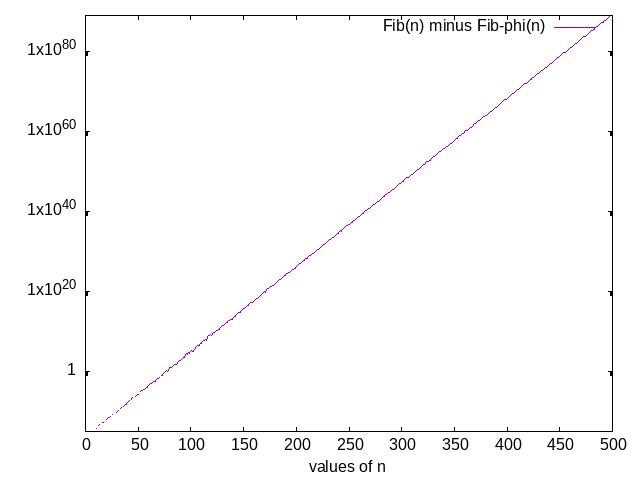
\includegraphics{fig/1-13.png}

\hypertarget{exercise-1.14}{%
\section{Exercise 1.14}\label{exercise-1.14}}

Below is the default version of the count-change function. I'll be
aggressively modifying it in order to get a graph out of it.

\hypertarget{count-change}{%
\label{count-change}}%
\begin{Shaded}
\begin{Highlighting}[numbers=left,,]
\NormalTok{(}\ExtensionTok{define}\FunctionTok{ }\NormalTok{(count{-}change amount)}
\NormalTok{  (cc amount }\DecValTok{5}\NormalTok{))}

\NormalTok{(}\ExtensionTok{define}\FunctionTok{ }\NormalTok{(cc amount kinds{-}of{-}coins)}
\NormalTok{  (}\KeywordTok{cond}\NormalTok{ ((}\OperatorTok{=}\NormalTok{ amount }\DecValTok{0}\NormalTok{) }\DecValTok{1}\NormalTok{)}
\NormalTok{        ((}\KeywordTok{or}\NormalTok{ (}\OperatorTok{\textless{}}\NormalTok{ amount }\DecValTok{0}\NormalTok{)}
\NormalTok{             (}\OperatorTok{=}\NormalTok{ kinds{-}of{-}coins }\DecValTok{0}\NormalTok{))}
         \DecValTok{0}\NormalTok{)}
\NormalTok{        (}\KeywordTok{else}
\NormalTok{         (}\OperatorTok{+}\NormalTok{ (cc amount (}\OperatorTok{{-}}\NormalTok{ kinds{-}of{-}coins }\DecValTok{1}\NormalTok{))}
\NormalTok{            (cc (}\OperatorTok{{-}}\NormalTok{ amount (first{-}denomination}
\NormalTok{                           kinds{-}of{-}coins))}
\NormalTok{                kinds{-}of{-}coins)))))}

\NormalTok{(}\ExtensionTok{define}\FunctionTok{ }\NormalTok{(first{-}denomination kinds{-}of{-}coins)}
\NormalTok{  (}\KeywordTok{cond}\NormalTok{ ((}\OperatorTok{=}\NormalTok{ kinds{-}of{-}coins }\DecValTok{1}\NormalTok{) }\DecValTok{1}\NormalTok{)}
\NormalTok{        ((}\OperatorTok{=}\NormalTok{ kinds{-}of{-}coins }\DecValTok{2}\NormalTok{) }\DecValTok{5}\NormalTok{)}
\NormalTok{        ((}\OperatorTok{=}\NormalTok{ kinds{-}of{-}coins }\DecValTok{3}\NormalTok{) }\DecValTok{10}\NormalTok{)}
\NormalTok{        ((}\OperatorTok{=}\NormalTok{ kinds{-}of{-}coins }\DecValTok{4}\NormalTok{) }\DecValTok{25}\NormalTok{)}
\NormalTok{        ((}\OperatorTok{=}\NormalTok{ kinds{-}of{-}coins }\DecValTok{5}\NormalTok{) }\DecValTok{50}\NormalTok{)))}
\end{Highlighting}
\end{Shaded}

\hypertarget{question-13}{%
\subsection{Question}\label{question-13}}

Draw the tree illustrating the process generated by the count-change
procedure of 1.2.2 in making change for 11 cents.

\hypertarget{answer-13}{%
\subsection{Answer}\label{answer-13}}

I want to generate this graph algorithmically.

\hypertarget{count-change-graphviz}{%
\label{count-change-graphviz}}%
\begin{Shaded}
\begin{Highlighting}[numbers=left,,]
\CommentTok{;; cursed global}
\NormalTok{(}\ExtensionTok{define}\FunctionTok{ bubblecounter }\DecValTok{0}\NormalTok{)}
\CommentTok{;; Returns \# of ways change can be made}
\CommentTok{;; "Helper" for (cc)}
\NormalTok{(}\ExtensionTok{define}\FunctionTok{ }\NormalTok{(count{-}change amount)}
\NormalTok{  (}\KeywordTok{display} \StringTok{"digraph \{}\CharTok{\textbackslash{}n}\StringTok{"}\NormalTok{) }\CommentTok{;; start graph}
\NormalTok{  (cc amount }\DecValTok{5} \DecValTok{0}\NormalTok{)}
\NormalTok{  (}\KeywordTok{display} \StringTok{"\}}\CharTok{\textbackslash{}n}\StringTok{"}\NormalTok{) }\CommentTok{;; end graph}
\NormalTok{  (}\KeywordTok{set!}\NormalTok{ bubblecounter }\DecValTok{0}\NormalTok{))}

\CommentTok{;; GraphViz output}
\CommentTok{;; Derivative: https://stackoverflow.com/a/14806144}
\NormalTok{(}\ExtensionTok{define}\FunctionTok{ }\NormalTok{(cc amount kinds{-}of{-}coins oldbubble)}
\NormalTok{  (}\KeywordTok{let}\NormalTok{ ((recur (}\KeywordTok{lambda}\NormalTok{ (new{-}amount new{-}kinds)}
\NormalTok{                 (}\KeywordTok{begin}
\NormalTok{                   (}\KeywordTok{display} \StringTok{"}\CharTok{\textbackslash{}"}\StringTok{"}\NormalTok{) }\CommentTok{;; Source bubble}
\NormalTok{                   (}\KeywordTok{display}\NormalTok{ \textasciigrave{}(,oldbubble ,amount ,kinds{-}of{-}coins))}
\NormalTok{                   (}\KeywordTok{display} \StringTok{"}\CharTok{\textbackslash{}"}\StringTok{"}\NormalTok{)}
\NormalTok{                   (}\KeywordTok{display} \StringTok{" {-}\textgreater{} "}\NormalTok{) }\CommentTok{;; arrow pointing from parent to child}
\NormalTok{                   (}\KeywordTok{display} \StringTok{"}\CharTok{\textbackslash{}"}\StringTok{"}\NormalTok{) }\CommentTok{;; child bubble}
\NormalTok{                   (}\KeywordTok{display}\NormalTok{ \textasciigrave{}(,bubblecounter ,new{-}amount ,new{-}kinds))}
\NormalTok{                   (}\KeywordTok{display} \StringTok{"}\CharTok{\textbackslash{}"}\StringTok{"}\NormalTok{)}
\NormalTok{                   (}\KeywordTok{display} \StringTok{"}\CharTok{\textbackslash{}n}\StringTok{"}\NormalTok{)}
\NormalTok{                   (cc new{-}amount new{-}kinds bubblecounter)))))}
\NormalTok{    (}\KeywordTok{set!}\NormalTok{ bubblecounter (}\OperatorTok{+}\NormalTok{ bubblecounter }\DecValTok{1}\NormalTok{))}
\NormalTok{    (}\KeywordTok{cond}\NormalTok{ ((}\OperatorTok{=}\NormalTok{ amount }\DecValTok{0}\NormalTok{) }\DecValTok{1}\NormalTok{)}
\NormalTok{          ((}\KeywordTok{or}\NormalTok{ (}\OperatorTok{\textless{}}\NormalTok{ amount }\DecValTok{0}\NormalTok{) (}\OperatorTok{=}\NormalTok{ kinds{-}of{-}coins }\DecValTok{0}\NormalTok{)) }\DecValTok{0}\NormalTok{)}
\NormalTok{          (}\KeywordTok{else}\NormalTok{ (}\OperatorTok{+}
\NormalTok{                 (recur amount (}\OperatorTok{{-}}\NormalTok{ kinds{-}of{-}coins }\DecValTok{1}\NormalTok{))}
\NormalTok{                 (recur (}\OperatorTok{{-}}\NormalTok{ amount}
\NormalTok{                           (first{-}denomination kinds{-}of{-}coins))}
\NormalTok{                        kinds{-}of{-}coins))))))}

\NormalTok{(}\ExtensionTok{define}\FunctionTok{ }\NormalTok{(first{-}denomination kinds{-}of{-}coins)}
\NormalTok{  (}\KeywordTok{cond}\NormalTok{ ((}\OperatorTok{=}\NormalTok{ kinds{-}of{-}coins }\DecValTok{1}\NormalTok{) }\DecValTok{1}\NormalTok{)}
\NormalTok{        ((}\OperatorTok{=}\NormalTok{ kinds{-}of{-}coins }\DecValTok{2}\NormalTok{) }\DecValTok{5}\NormalTok{)}
\NormalTok{        ((}\OperatorTok{=}\NormalTok{ kinds{-}of{-}coins }\DecValTok{3}\NormalTok{) }\DecValTok{10}\NormalTok{)}
\NormalTok{        ((}\OperatorTok{=}\NormalTok{ kinds{-}of{-}coins }\DecValTok{4}\NormalTok{) }\DecValTok{25}\NormalTok{)}
\NormalTok{        ((}\OperatorTok{=}\NormalTok{ kinds{-}of{-}coins }\DecValTok{5}\NormalTok{) }\DecValTok{50}\NormalTok{)))}
\end{Highlighting}
\end{Shaded}

I'm not going to include the full printout of the
\texttt{(count-change\ 11)}, here's an example of what this looks like
via \texttt{1}.

\hypertarget{count-change-test}{%
\label{count-change-test}}%
\begin{Shaded}
\begin{Highlighting}[numbers=left,,]
\NormalTok{\textless{}\textless{}count{-}change{-}graphviz\textgreater{}\textgreater{}}
\NormalTok{(count{-}change }\DecValTok{1}\NormalTok{)}
\end{Highlighting}
\end{Shaded}

\begin{Shaded}
\begin{Highlighting}[]
\KeywordTok{digraph} \OtherTok{\{}
\StringTok{"(0 1 5)"}\CommentTok{ }\OtherTok{{-}\textgreater{}}\CommentTok{ }\StringTok{"(1 1 4)"}
\StringTok{"(1 1 4)"}\CommentTok{ }\OtherTok{{-}\textgreater{}}\CommentTok{ }\StringTok{"(2 1 3)"}
\StringTok{"(2 1 3)"}\CommentTok{ }\OtherTok{{-}\textgreater{}}\CommentTok{ }\StringTok{"(3 1 2)"}
\StringTok{"(3 1 2)"}\CommentTok{ }\OtherTok{{-}\textgreater{}}\CommentTok{ }\StringTok{"(4 1 1)"}
\StringTok{"(4 1 1)"}\CommentTok{ }\OtherTok{{-}\textgreater{}}\CommentTok{ }\StringTok{"(5 1 0)"}
\StringTok{"(4 1 1)"}\CommentTok{ }\OtherTok{{-}\textgreater{}}\CommentTok{ }\StringTok{"(6 0 1)"}
\StringTok{"(3 1 2)"}\CommentTok{ }\OtherTok{{-}\textgreater{}}\CommentTok{ }\StringTok{"(7 {-}4 2)"}
\StringTok{"(2 1 3)"}\CommentTok{ }\OtherTok{{-}\textgreater{}}\CommentTok{ }\StringTok{"(8 {-}9 3)"}
\StringTok{"(1 1 4)"}\CommentTok{ }\OtherTok{{-}\textgreater{}}\CommentTok{ }\StringTok{"(9 {-}24 4)"}
\StringTok{"(0 1 5)"}\CommentTok{ }\OtherTok{{-}\textgreater{}}\CommentTok{ }\StringTok{"(10 {-}49 5)"}
\OtherTok{\}}
\end{Highlighting}
\end{Shaded}

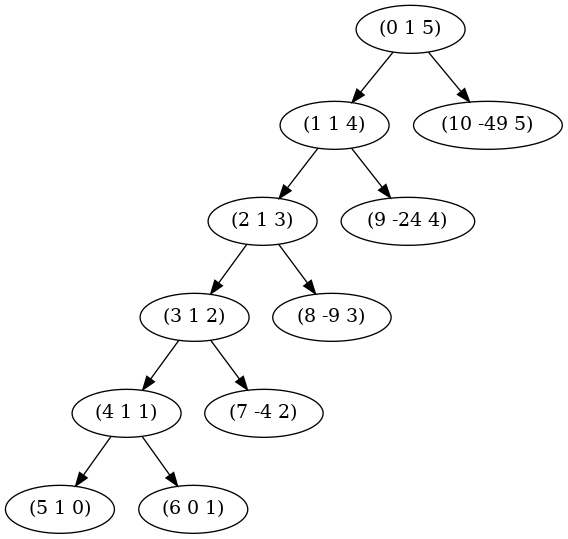
\includegraphics{fig/cc-test.png}

So, the graph of \texttt{(count-change\ 11)} is:

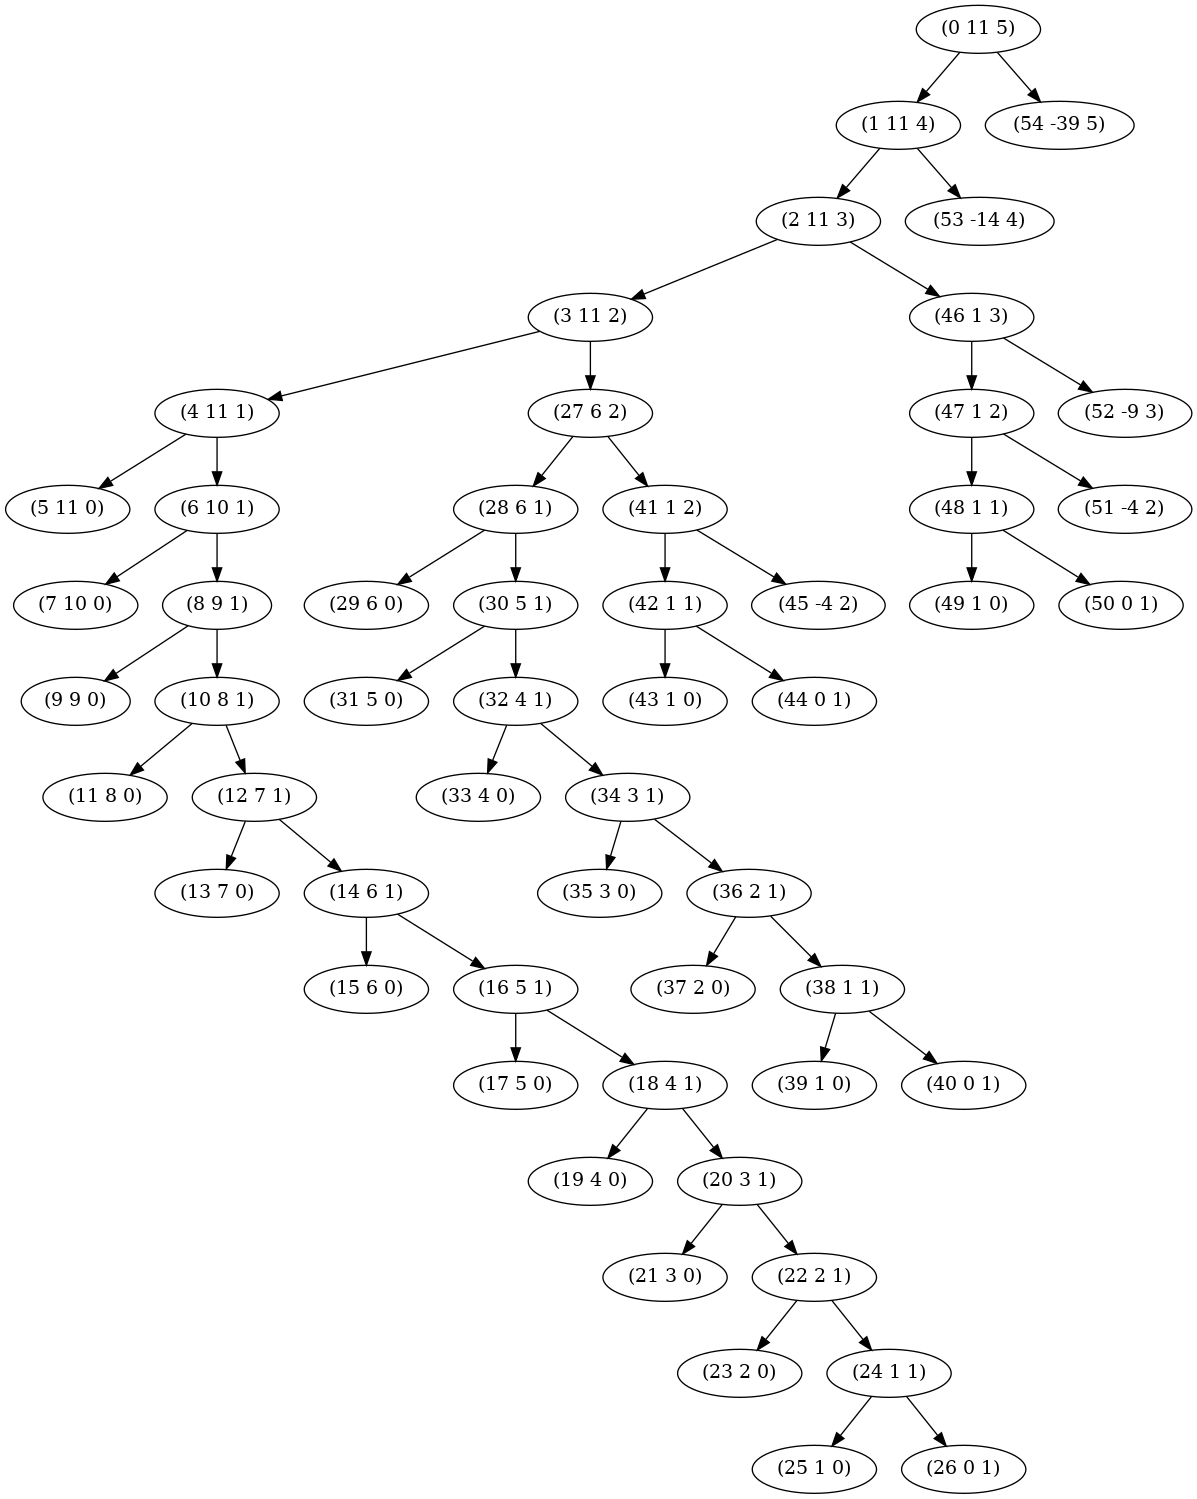
\includegraphics{fig/cc-11.png}

\hypertarget{question-2-1}{%
\subsection{Question 2}\label{question-2-1}}

What are the orders of growth of the space and number of steps used by
this process as the amount to be changed increases?

\hypertarget{answer-2-1}{%
\subsection{Answer 2}\label{answer-2-1}}

Let's look at this via the number of function calls needed for value
\texttt{n}. Instead of returning an integer, I'll return a pair where
\texttt{car} is the number of ways to count change, and \texttt{cdr} is
the number of function calls that have occurred down that branch of the
tree.

\hypertarget{cc-calls}{%
\label{cc-calls}}%
\begin{Shaded}
\begin{Highlighting}[numbers=left,,]
\NormalTok{(}\ExtensionTok{define}\FunctionTok{ }\NormalTok{(count{-}calls amount)}
\NormalTok{  (cc{-}calls amount }\DecValTok{5}\NormalTok{))}

\NormalTok{(}\ExtensionTok{define}\FunctionTok{ }\NormalTok{(cc{-}calls amount kinds{-}of{-}coins)}
\NormalTok{  (}\KeywordTok{cond}\NormalTok{ ((}\OperatorTok{=}\NormalTok{ amount }\DecValTok{0}\NormalTok{) \textquotesingle{}(}\DecValTok{1} \OperatorTok{.} \DecValTok{1}\NormalTok{))}
\NormalTok{        ((}\KeywordTok{or}\NormalTok{ (}\OperatorTok{\textless{}}\NormalTok{ amount }\DecValTok{0}\NormalTok{)}
\NormalTok{             (}\OperatorTok{=}\NormalTok{ kinds{-}of{-}coins }\DecValTok{0}\NormalTok{))}
\NormalTok{         \textquotesingle{}(}\DecValTok{0} \OperatorTok{.} \DecValTok{1}\NormalTok{))}
\NormalTok{        (}\KeywordTok{else}
\NormalTok{         (}\KeywordTok{let}\NormalTok{ ((a (cc{-}calls amount (}\OperatorTok{{-}}\NormalTok{ kinds{-}of{-}coins }\DecValTok{1}\NormalTok{)))}
\NormalTok{               (b (cc{-}calls (}\OperatorTok{{-}}\NormalTok{ amount (first{-}denomination}
\NormalTok{                                 kinds{-}of{-}coins))}
\NormalTok{                      kinds{-}of{-}coins)))}
\NormalTok{           (}\KeywordTok{cons}\NormalTok{ (}\OperatorTok{+}\NormalTok{ (}\KeywordTok{car}\NormalTok{ a)}
\NormalTok{                    (}\KeywordTok{car}\NormalTok{ b))}
\NormalTok{                 (}\OperatorTok{+} \DecValTok{1}
\NormalTok{                    (}\KeywordTok{cdr}\NormalTok{ a)}
\NormalTok{                    (}\KeywordTok{cdr}\NormalTok{ b)))))))}

\NormalTok{(}\ExtensionTok{define}\FunctionTok{ }\NormalTok{(first{-}denomination kinds{-}of{-}coins)}
\NormalTok{  (}\KeywordTok{cond}\NormalTok{ ((}\OperatorTok{=}\NormalTok{ kinds{-}of{-}coins }\DecValTok{1}\NormalTok{) }\DecValTok{1}\NormalTok{)}
\NormalTok{        ((}\OperatorTok{=}\NormalTok{ kinds{-}of{-}coins }\DecValTok{2}\NormalTok{) }\DecValTok{5}\NormalTok{)}
\NormalTok{        ((}\OperatorTok{=}\NormalTok{ kinds{-}of{-}coins }\DecValTok{3}\NormalTok{) }\DecValTok{10}\NormalTok{)}
\NormalTok{        ((}\OperatorTok{=}\NormalTok{ kinds{-}of{-}coins }\DecValTok{4}\NormalTok{) }\DecValTok{25}\NormalTok{)}
\NormalTok{        ((}\OperatorTok{=}\NormalTok{ kinds{-}of{-}coins }\DecValTok{5}\NormalTok{) }\DecValTok{50}\NormalTok{)))}
\end{Highlighting}
\end{Shaded}

\begin{longtable}[]{@{}lll@{}}
\toprule
\endhead
1 & 1 & (1 . 11) \\
2 & 1 & (1 . 13) \\
3 & 1 & (1 . 15) \\
4 & 1 & (1 . 17) \\
5 & 2 & (2 . 19) \\
6 & 2 & (2 . 25) \\
7 & 2 & (2 . 29) \\
8 & 2 & (2 . 33) \\
9 & 2 & (2 . 37) \\
10 & 4 & (4 . 41) \\
\bottomrule
\end{longtable}

\hypertarget{cc-calls-100}{%
\label{cc-calls-100}}%
\begin{Shaded}
\begin{Highlighting}[numbers=left,,]
\NormalTok{(use{-}srfis \textquotesingle{}(}\DecValTok{1}\NormalTok{))}
\NormalTok{\textless{}\textless{}cc{-}calls\textgreater{}\textgreater{}}
\NormalTok{(}\KeywordTok{let*}\NormalTok{ ((vals (drop (iota }\DecValTok{101}\NormalTok{) }\DecValTok{1}\NormalTok{))}
\NormalTok{       (mine (map count{-}calls vals)))}
\NormalTok{  (zip vals (map }\KeywordTok{car}\NormalTok{ mine) (map }\KeywordTok{cdr}\NormalTok{ mine)))}
\end{Highlighting}
\end{Shaded}

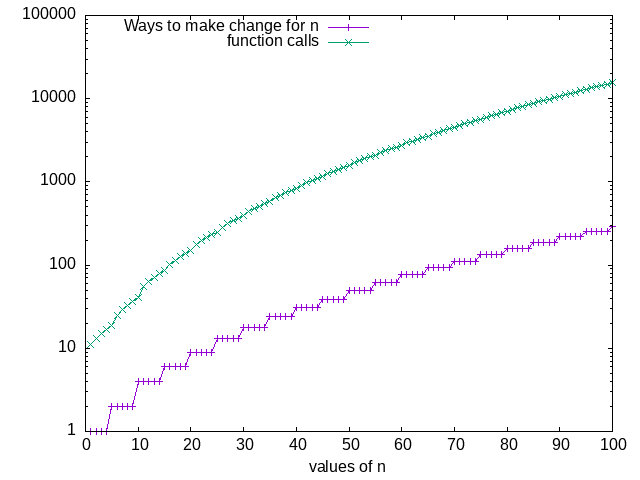
\includegraphics{fig/cc-100.png}

I believe the space to be \(\Theta(n+d)\) as the function calls count
down the denominations before counting down the change. However I notice
most answers describe \(\Theta(n)\) instead, maybe I'm being overly
pedantic and getting the wrong answer.

My issues came finding the time. The book describes the meaning and
properties of \(\Theta\) notation in
\href{http://sarabander.github.io/sicp/html/1_002e2.xhtml\#g_t1_002e2_002e3}{Section
1.2.3}. However, my lack of formal math education made realizing the
significance of this passage difficult. For one, I didn't understand
that \(k_{1}f(n) \leq R(n) \leq k_{2}f(n)\) means "you can find the
\(\Theta\) by proving that a graph of the algorithm's resource usage is
bounded by two identical functions multiplied by constants." So, the
graph of resource usage for an algorithm with \(\Theta(n^{2})\) will by
bounded by lines of \(n^{2} \times some constant\), the top boundary's
constant being larger than the small boundary. These are arbitrarily
chosen constants, you're just proving that the function behaves the way
you think it does.

Overall, finding the \(\Theta\) and \(\Omega\) and \(O\) notations (they
are all different btw!) is about aggressively simplifying to make a very
general statement about the behavior of the algorithm.

I could tell that a "correct" way to find the \(\Theta\) would be to
make a formula which describes the algorithm's function calls for given
input and denominations. This is one of the biggest time sinks, although
I had a lot of fun and learned a lot. In the end, with some help from
Jach in a Lisp Discord, I had the following formula:

\[
\sum_{i=1}^{ceil(n / val(d))} T(n - val(d)*i, d)
\]

But I wasn't sure where to go from here. The graphs let me see some
interesting trends, though I didn't get any closer to an answer in the
process.

By reading on other websites, I knew that you could find \(\Theta\) by
obtaining a formula for \(R(n)\) and removing constants to end up with a
term of interest. For example, if your algorithm's resource usage is
\(\frac{n^{2} + 7n}{5}\), this demonstrates \(\Theta(n^{2})\). So I know
a formula \textbf{without} a \(\sum\) would give me the answer I wanted.
It didn't occur to me that it might be possible to use calculus to
remove the \(\sum\) from the equation. At this point I knew I was stuck
and decided to look up a guide.

After seeing a few solutions that I found somewhat confusing, I landed
on \href{https://codology.net/post/sicp-solution-exercise-1-14/}{this
awesome article from Codology.net}. They show how you can remove the
summation, and proposed this equation for count-change with 5
denominations:

\[
T(n,5)=\frac n{50}+1+\sum_{i=0}^{n/50}T(n-50i,1)
\]

Which, when expanded and simplified, demonstrates \(\Theta(n^{5})\) for
5 denominations.

Overall I'm relieved that I wasn't entirely off, given I haven't done
math work like this since college. It's inspired me to restart my
remedial math courses, I don't think I really grasped the nature of math
as a tool of empowerment until now.

\hypertarget{exercise-1.15}{%
\section{Exercise 1.15}\label{exercise-1.15}}

\hypertarget{question-1-1}{%
\subsection{Question 1}\label{question-1-1}}

The sine of an angle (specified in radians) can be computed by making
use of the approximation \(\sin x ≈ x\) if \(x\) is sufficiently small,
and the trigonometric identity
\(\sin x = 3\sin\frac{x}{3} − 4\sin^3\frac{x}{3}\) to reduce the size of
the argument of sin. (For purposes of this exercise an angle is
considered ``sufficiently small'' if its magnitude is not greater than
0.1 radians.) These ideas are incorporated in the following procedures:

\hypertarget{1-15-deps}{%
\label{1-15-deps}}%
\begin{Shaded}
\begin{Highlighting}[numbers=left,,]
\NormalTok{(}\ExtensionTok{define}\FunctionTok{ }\NormalTok{(cube x) (}\OperatorTok{*}\NormalTok{ x x x))}
\NormalTok{(}\ExtensionTok{define}\FunctionTok{ }\NormalTok{(p x) (}\OperatorTok{{-}}\NormalTok{ (}\OperatorTok{*} \DecValTok{3}\NormalTok{ x) (}\OperatorTok{*} \DecValTok{4}\NormalTok{ (cube x))))}
\NormalTok{(}\ExtensionTok{define}\FunctionTok{ }\NormalTok{(sine }\KeywordTok{angle}\NormalTok{)}
\NormalTok{  (}\KeywordTok{if}\NormalTok{ (}\KeywordTok{not}\NormalTok{ (}\OperatorTok{\textgreater{}}\NormalTok{ (}\KeywordTok{abs} \KeywordTok{angle}\NormalTok{) }\FloatTok{0.1}\NormalTok{))}
      \KeywordTok{angle}
\NormalTok{      (p (sine (}\OperatorTok{/} \KeywordTok{angle} \FloatTok{3.0}\NormalTok{)))))}
\end{Highlighting}
\end{Shaded}

How many times is the procedure \texttt{p} applied when
\VERB|\NormalTok{(sine }\FloatTok{12.15}\NormalTok{)}| is evaluated?

\hypertarget{answer-1-1}{%
\subsection{Answer 1}\label{answer-1-1}}

Let's find out!

\hypertarget{1-15-p-measure}{%
\label{1-15-p-measure}}%
\begin{Shaded}
\begin{Highlighting}[numbers=left,,]
\NormalTok{(}\ExtensionTok{define}\FunctionTok{ }\NormalTok{(cube x) (}\OperatorTok{*}\NormalTok{ x x x))}
\NormalTok{(}\ExtensionTok{define}\FunctionTok{ }\NormalTok{(p x) (}\OperatorTok{{-}}\NormalTok{ (}\OperatorTok{*} \DecValTok{3}\NormalTok{ x) (}\OperatorTok{*} \DecValTok{4}\NormalTok{ (cube x))))}
\NormalTok{(}\ExtensionTok{define}\FunctionTok{ }\NormalTok{(sine }\KeywordTok{angle}\NormalTok{)}
\NormalTok{  (}\KeywordTok{if}\NormalTok{ (}\KeywordTok{not}\NormalTok{ (}\OperatorTok{\textgreater{}}\NormalTok{ (}\KeywordTok{abs} \KeywordTok{angle}\NormalTok{) }\FloatTok{0.1}\NormalTok{))}
\NormalTok{      (}\KeywordTok{cons} \KeywordTok{angle} \DecValTok{0}\NormalTok{)}
\NormalTok{      (}\KeywordTok{let}\NormalTok{ ((x (sine (}\OperatorTok{/} \KeywordTok{angle} \FloatTok{3.0}\NormalTok{))))}
\NormalTok{        (}\KeywordTok{cons}\NormalTok{ (p (}\KeywordTok{car}\NormalTok{ x)) (}\OperatorTok{+} \DecValTok{1}\NormalTok{ (}\KeywordTok{cdr}\NormalTok{ x))))))}
\end{Highlighting}
\end{Shaded}

\hypertarget{1-15-sine1215}{%
\label{1-15-sine1215}}%
\begin{Shaded}
\begin{Highlighting}[numbers=left,,]
\NormalTok{\textless{}\textless{}1{-}15{-}p{-}measure\textgreater{}\textgreater{}}
\NormalTok{(}\KeywordTok{let}\NormalTok{ ((xy (sine }\FloatTok{12.15}\NormalTok{)))}
\NormalTok{  (}\KeywordTok{list}\NormalTok{ (}\KeywordTok{car}\NormalTok{ xy) (}\KeywordTok{cdr}\NormalTok{ xy)))}
\end{Highlighting}
\end{Shaded}

\begin{longtable}[]{@{}ll@{}}
\toprule
\endhead
-0.39980345741334 & 5 \\
\bottomrule
\end{longtable}

\texttt{p} is evaluated 5 times.

\hypertarget{question-2-2}{%
\subsection{Question 2}\label{question-2-2}}

What is the order of growth in space and number of steps (as a function
of \texttt{a}) used by the process generated by the sine procedure when
\VERB|\NormalTok{(sine a)}| is evaluated?

\hypertarget{answer-2-2}{%
\subsection{Answer 2}\label{answer-2-2}}

\hypertarget{1-15-tab1}{%
\label{1-15-tab1}}%
\begin{Shaded}
\begin{Highlighting}[numbers=left,,]
\NormalTok{(use{-}srfis \textquotesingle{}(}\DecValTok{1}\NormalTok{))}
\NormalTok{\textless{}\textless{}1{-}15{-}p{-}measure\textgreater{}\textgreater{}}
\NormalTok{(}\KeywordTok{let*}\NormalTok{ ((vals (iota }\DecValTok{300} \FloatTok{0.1} \FloatTok{0.1}\NormalTok{))}
\NormalTok{       (sines (map (λ (i)}
\NormalTok{                     (}\KeywordTok{cdr}\NormalTok{ (sine i)))}
\NormalTok{                   vals)))}
\NormalTok{  (zip vals sines))}
\end{Highlighting}
\end{Shaded}

Example output:

\begin{longtable}[]{@{}ll@{}}
\toprule
\endhead
0.1 & 0 \\
0.2 & 1 \\
0.30000000000000004 & 2 \\
0.4 & 2 \\
0.5 & 2 \\
0.6 & 2 \\
0.7000000000000001 & 2 \\
0.8 & 2 \\
0.9 & 2 \\
1.0 & 3 \\
\bottomrule
\end{longtable}

\begin{Shaded}
\begin{Highlighting}[]
\NormalTok{reset \# helps with various issues in execution}
\NormalTok{set xlabel \textquotesingle{}values of x\textquotesingle{}}
\NormalTok{set logscale x}
\NormalTok{set key top left}
\NormalTok{set style fill solid 1.00 border}
\NormalTok{set style function fillsteps below}

\NormalTok{f(x) = log(x) + 2.3}

\NormalTok{plot data using 1:2 with fillsteps title \textquotesingle{}function calls\textquotesingle{}, \textbackslash{}}
\NormalTok{     data using 1:(f($1)) with lines title \textquotesingle{}log(x) + 2. 3\textquotesingle{}}
\end{Highlighting}
\end{Shaded}

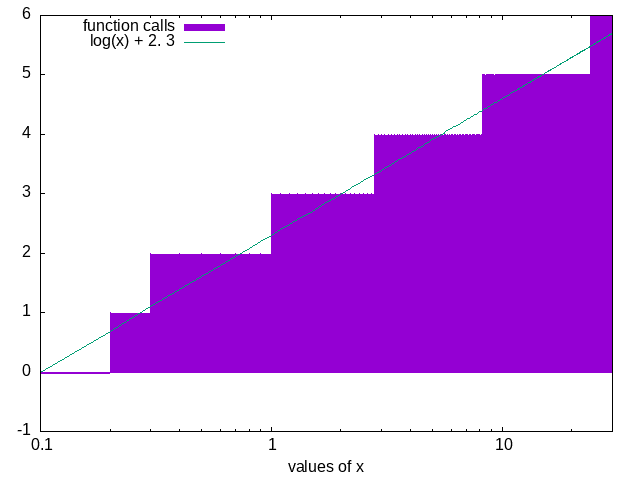
\includegraphics{fig/1-15-step.png}

This graph shows that the number of times \texttt{sine} will be called
is logarithmic.

\begin{itemize}
\tightlist
\item
  0.1 to 0.2 are divided once
\item
  0.3 to 0.8 are divided twice
\item
  0.9 to 2.6 are divided three times
\item
  2.7 to 8 are divided four times
\item
  8.5 to 23.8 are divided five times
\end{itemize}

Given that the calls to \texttt{p} get stacked recursively, like this:

\begin{Shaded}
\begin{Highlighting}[]
\NormalTok{(sine }\FloatTok{12.15}\NormalTok{)}
\NormalTok{(p (sine }\FloatTok{4.05}\NormalTok{))}
\NormalTok{(p (p (sine }\FloatTok{1.35}\NormalTok{)))}
\NormalTok{(p (p (p (sine }\FloatTok{0.45}\NormalTok{))))}
\NormalTok{(p (p (p (p (sine }\FloatTok{0.15}\NormalTok{)))))}
\NormalTok{(p (p (p (p (p (sine }\FloatTok{0.05}\NormalTok{))))))}
\NormalTok{(p (p (p (p (p }\FloatTok{0.05}\NormalTok{)))))}
\NormalTok{(p (p (p (p }\FloatTok{0.14950000000000002}\NormalTok{))))}
\NormalTok{(p (p (p }\FloatTok{0.43513455050000005}\NormalTok{)))}
\NormalTok{(p (p }\FloatTok{0.9758465331678772}\NormalTok{))}
\NormalTok{(p {-}}\FloatTok{0.7895631144708228}\NormalTok{)}
\NormalTok{{-}}\FloatTok{0.39980345741334}
\end{Highlighting}
\end{Shaded}

So I argue the space and time is \(\Theta(\log(n))\)

We can also prove this for the time by benchmarking the function:

\hypertarget{1-15-sine-bench}{%
\label{1-15-sine-bench}}%
\begin{Shaded}
\begin{Highlighting}[numbers=left,,]
\CommentTok{;; This execution takes too long for org{-}mode, so I\textquotesingle{}m doing it}
\CommentTok{;; externally and importing the results}
\NormalTok{(use{-}srfis \textquotesingle{}(}\DecValTok{1}\NormalTok{))}
\NormalTok{(use{-}modules (ice{-}9 format))}
\NormalTok{(}\KeywordTok{load} \StringTok{"../../mattbench.scm"}\NormalTok{)}
\NormalTok{\textless{}\textless{}1{-}15{-}deps\textgreater{}\textgreater{}}
\NormalTok{(}\KeywordTok{let*}\NormalTok{ ((vals (iota }\DecValTok{300} \FloatTok{0.1} \FloatTok{0.1}\NormalTok{))}
\NormalTok{       (times (map (λ (i)}
\NormalTok{                     (mattbench (λ () (sine i)) }\DecValTok{1000000}\NormalTok{))}
\NormalTok{                   vals)))}
\NormalTok{  (}\KeywordTok{with{-}output{-}to{-}file} \StringTok{"sine{-}bench.dat"}\NormalTok{ (λ ()}
\NormalTok{     (map (λ (x y)}
\NormalTok{           (format }\DecValTok{\#t} \StringTok{"\textasciitilde{}s\textasciitilde{}/\textasciitilde{}s\textasciitilde{}\%"}\NormalTok{ x y))}
\NormalTok{         vals times))))}
\end{Highlighting}
\end{Shaded}

\begin{Shaded}
\begin{Highlighting}[]
\NormalTok{reset \# helps with various issues in execution}
\NormalTok{set xtics 0.5}
\NormalTok{set xlabel \textquotesingle{}values of x\textquotesingle{}}
\NormalTok{set logscale x}
\NormalTok{set key top left}
\NormalTok{set style fill solid 1.00 border}
\NormalTok{\#set style function fillsteps below}

\NormalTok{f(x) = (log(x) * a) + b}
\NormalTok{fit f(x) \textquotesingle{}Ex15/sine{-}bench.dat\textquotesingle{} using 1:2 via a,b}

\NormalTok{plot \textquotesingle{}Ex15/sine{-}bench.dat\textquotesingle{} using 1:2 with fillsteps title \textquotesingle{}time to execute\textquotesingle{}, \textbackslash{}}
\NormalTok{     \textquotesingle{}Ex15/sine{-}bench.dat\textquotesingle{} using 1:(f($1)) with lines title sprintf(\textquotesingle{}(log(x) * \%.2f) + \%.2f\textquotesingle{}, a, b)}
\end{Highlighting}
\end{Shaded}

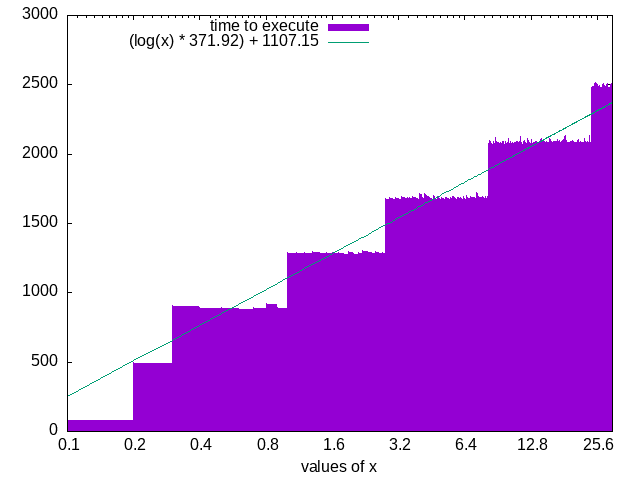
\includegraphics{fig/1-15-bench.png}

\hypertarget{exercise-1.16}{%
\section{Exercise 1.16}\label{exercise-1.16}}

\hypertarget{text-2}{%
\subsection{Text}\label{text-2}}

\hypertarget{txt-expt}{%
\label{txt-expt}}%
\begin{Shaded}
\begin{Highlighting}[numbers=left,,]
\NormalTok{(}\ExtensionTok{define}\FunctionTok{ }\NormalTok{(expt{-}rec b n)}
\NormalTok{  (}\KeywordTok{if}\NormalTok{ (}\OperatorTok{=}\NormalTok{ n }\DecValTok{0}\NormalTok{) }
      \DecValTok{1} 
\NormalTok{      (}\OperatorTok{*}\NormalTok{ b (expt{-}rec b (}\OperatorTok{{-}}\NormalTok{ n }\DecValTok{1}\NormalTok{)))))}

\NormalTok{(}\ExtensionTok{define}\FunctionTok{ }\NormalTok{(expt{-}iter b n) }
\NormalTok{  (}\ExtensionTok{define}\FunctionTok{ }\NormalTok{(iter counter product)}
\NormalTok{    (}\KeywordTok{if}\NormalTok{ (}\OperatorTok{=}\NormalTok{ counter }\DecValTok{0}\NormalTok{)}
\NormalTok{        product}
\NormalTok{        (iter (}\OperatorTok{{-}}\NormalTok{ counter }\DecValTok{1}\NormalTok{)}
\NormalTok{              (}\OperatorTok{*}\NormalTok{ b product))))}
\NormalTok{  (iter n }\DecValTok{1}\NormalTok{))}

\NormalTok{(}\ExtensionTok{define}\FunctionTok{ }\NormalTok{(fast{-}expt b n)}
\NormalTok{  (}\KeywordTok{cond}\NormalTok{ ((}\OperatorTok{=}\NormalTok{ n }\DecValTok{0}\NormalTok{) }
         \DecValTok{1}\NormalTok{)}
\NormalTok{        ((}\KeywordTok{even?}\NormalTok{ n) }
\NormalTok{         (square (fast{-}expt b (}\OperatorTok{/}\NormalTok{ n }\DecValTok{2}\NormalTok{))))}
\NormalTok{        (}\KeywordTok{else} 
\NormalTok{         (}\OperatorTok{*}\NormalTok{ b (fast{-}expt b (}\OperatorTok{{-}}\NormalTok{ n }\DecValTok{1}\NormalTok{))))))}
\end{Highlighting}
\end{Shaded}

\hypertarget{question-14}{%
\subsection{Question}\label{question-14}}

Design a procedure that evolves an iterative exponentiation process that
uses successive squaring and uses a logarithmic number of steps, as does
fast-expt. (Hint: Using the observation that
\((b^{n/2})^2=(b^2)^{n/2}\), keep, along with the exponent \(n\) and the
base \(b\), an additional state variable \(a\) , and define the state
transformation in such a way that the product \({ab}^n\) is unchanged
from state to state. At the beginning of the process \(a\) is taken to
be 1, and the answer is given by the value of \(a\) at the end of the
process. In general, the technique of defining an \emph{invariant
quantity} that remains unchanged from state to state is a powerful way
to think about the design of iterative algorithms.)

\hypertarget{diary-2}{%
\subsection{Diary}\label{diary-2}}

First I made this program which tries to use a false equivalence:
\[ab^2 = (a + 1)b^{n - 1}\]

\hypertarget{fast-expt-iter-fail1}{%
\label{fast-expt-iter-fail1}}%
\begin{Shaded}
\begin{Highlighting}[numbers=left,,]
\NormalTok{\textless{}\textless{}square\textgreater{}\textgreater{}}
\NormalTok{(}\ExtensionTok{define}\FunctionTok{ }\NormalTok{(fast{-}expt{-}iter b n)}
\NormalTok{  (}\ExtensionTok{define}\FunctionTok{ }\NormalTok{(iter b n a)}
\NormalTok{    (format }\DecValTok{\#t} \StringTok{"\textasciitilde{}\&|\textasciitilde{}s\textasciitilde{}/\textasciitilde{}/|\textasciitilde{}s\textasciitilde{}/\textasciitilde{}/|\textasciitilde{}s|\textasciitilde{}\%"}\NormalTok{ b n a)}
\NormalTok{    (}\KeywordTok{cond}\NormalTok{ ((}\OperatorTok{=}\NormalTok{ n }\DecValTok{1}\NormalTok{) (}\KeywordTok{begin}\NormalTok{ (format }\DecValTok{\#t} \StringTok{"\textasciitilde{}\&|\textasciitilde{}s\textasciitilde{}/\textasciitilde{}/|\textasciitilde{}s\textasciitilde{}/\textasciitilde{}/|\textasciitilde{}s|\textasciitilde{}\%"}\NormalTok{ (}\OperatorTok{*}\NormalTok{ b a) }\DecValTok{1} \DecValTok{1}\NormalTok{)}
\NormalTok{                          (}\OperatorTok{*}\NormalTok{ b a)))}
\NormalTok{          ((}\KeywordTok{even?}\NormalTok{ n) (iter (square b)}
\NormalTok{                         (}\OperatorTok{/}\NormalTok{ n }\DecValTok{2}\NormalTok{)}
\NormalTok{                         a))}
\NormalTok{          (}\KeywordTok{else}\NormalTok{ (iter b (}\OperatorTok{{-}}\NormalTok{ n }\DecValTok{1}\NormalTok{) (}\OperatorTok{+}\NormalTok{ a }\DecValTok{1}\NormalTok{)))))}
\NormalTok{  (format }\DecValTok{\#t} \StringTok{"|\textasciitilde{}a\textasciitilde{}/|\textasciitilde{}a\textasciitilde{}/|\textasciitilde{}a|\textasciitilde{}\%"} \StringTok{"base"} \StringTok{"power"} \StringTok{"variable"}\NormalTok{)}
\NormalTok{  (format }\DecValTok{\#t} \StringTok{"\textasciitilde{}\&|{-}{-}|{-}{-}|{-}{-}|\textasciitilde{}\%"}\NormalTok{)}
\NormalTok{  (iter b n }\DecValTok{1}\NormalTok{))}
\end{Highlighting}
\end{Shaded}

\begin{Shaded}
\begin{Highlighting}[numbers=left,,]
\NormalTok{\textless{}\textless{}fast{-}expt{-}iter{-}fail1\textgreater{}\textgreater{}}
\NormalTok{\textless{}\textless{}try{-}these\textgreater{}\textgreater{}}
\NormalTok{(fast{-}expt{-}iter }\DecValTok{2} \DecValTok{6}\NormalTok{)}
\end{Highlighting}
\end{Shaded}

Here's what the internal state looks like during \(2^6\) (correct answer
is 64):

\begin{longtable}[]{@{}lll@{}}
\toprule
base & power & variable \\
\midrule
\endhead
2 & 6 & 1 \\
4 & 3 & 1 \\
4 & 2 & 2 \\
16 & 1 & 2 \\
32 & 1 & 1 \\
\bottomrule
\end{longtable}

\hypertarget{answer-14}{%
\subsection{Answer}\label{answer-14}}

There are two key transforms to a faster algorithm. The first was
already shown in the text:

\[
    ab^n \to a(b^2)^{n/2}
\]

The second which I needed to deduce was this:

\[
    ab^n \to ((a \times b) \times b)^{n - 1}
\]

The solution essentially follows this logic:

\begin{itemize}
\tightlist
\item
  initialize \(a\) to 1
\item
  If \( n \) is 1, return \(b * a\)
\item
  else if \(n\) is even, halve \(n\), square \(b\), and iterate
\item
  else \(n\) is odd, so subtract 1 from \(n\) and \(a \to a \times b\)
\end{itemize}

\hypertarget{fast-expt-iter}{%
\label{fast-expt-iter}}%
\begin{Shaded}
\begin{Highlighting}[numbers=left,,]
\NormalTok{\textless{}\textless{}square\textgreater{}\textgreater{}}
\NormalTok{(}\ExtensionTok{define}\FunctionTok{ }\NormalTok{(fast{-}expt{-}iter b n)}
\NormalTok{  (}\ExtensionTok{define}\FunctionTok{ }\NormalTok{(iter b n a)}
\NormalTok{    (}\KeywordTok{cond}\NormalTok{ ((}\OperatorTok{=}\NormalTok{ n }\DecValTok{1}\NormalTok{) (}\OperatorTok{*}\NormalTok{ b a))}
\NormalTok{          ((}\KeywordTok{even?}\NormalTok{ n) (iter (square b)}
\NormalTok{                         (}\OperatorTok{/}\NormalTok{ n }\DecValTok{2}\NormalTok{)}
\NormalTok{                         a))}
\NormalTok{          (}\KeywordTok{else}\NormalTok{ (iter b (}\OperatorTok{{-}}\NormalTok{ n }\DecValTok{1}\NormalTok{) (}\OperatorTok{*}\NormalTok{ b a)))))}
\NormalTok{  (iter b n }\DecValTok{1}\NormalTok{))}
\end{Highlighting}
\end{Shaded}

\begin{longtable}[]{@{}ll@{}}
\toprule
\endhead
1 & 3 \\
2 & 9 \\
3 & 27 \\
4 & 81 \\
5 & 243 \\
6 & 729 \\
7 & 2187 \\
8 & 6561 \\
9 & 19683 \\
10 & 59049 \\
\bottomrule
\end{longtable}

\hypertarget{exercise-1.17}{%
\section{Exercise 1.17}\label{exercise-1.17}}

\hypertarget{question-15}{%
\subsection{Question}\label{question-15}}

The exponentiation algorithms in this section are based on performing
exponentiation by means of repeated multiplication. In a similar way,
one can perform integer multiplication by means of repeated addition.
The following multiplication procedure (in which it is assumed that our
language can only add, not multiply) is analogous to the expt procedure:

\begin{Shaded}
\begin{Highlighting}[numbers=left,,]
\NormalTok{(}\ExtensionTok{define}\FunctionTok{ }\NormalTok{(}\OperatorTok{*}\NormalTok{ a b)}
\NormalTok{  (}\KeywordTok{if}\NormalTok{ (}\OperatorTok{=}\NormalTok{ b }\DecValTok{0}\NormalTok{)}
      \DecValTok{0}
\NormalTok{      (}\OperatorTok{+}\NormalTok{ a (}\OperatorTok{*}\NormalTok{ a (}\OperatorTok{{-}}\NormalTok{ b }\DecValTok{1}\NormalTok{)))))}
\end{Highlighting}
\end{Shaded}

This algorithm takes a number of steps that is linear in \( b \). Now
suppose we include, together with addition, operations double, which
doubles an integer, and halve, which divides an (even) integer by 2.
Using these, design a multiplication procedure analogous to fast-expt
that uses a logarithmic number of steps.

\hypertarget{answer-15}{%
\subsection{Answer}\label{answer-15}}

\hypertarget{fast-mult-rec}{%
\label{fast-mult-rec}}%
\begin{Shaded}
\begin{Highlighting}[numbers=left,,]
\NormalTok{(}\ExtensionTok{define}\FunctionTok{ }\NormalTok{(double x)}
\NormalTok{  (}\OperatorTok{+}\NormalTok{ x x))}
\NormalTok{(}\ExtensionTok{define}\FunctionTok{ }\NormalTok{(halve x)}
\NormalTok{  (}\OperatorTok{/}\NormalTok{ x }\DecValTok{2}\NormalTok{))}
\NormalTok{(}\ExtensionTok{define}\FunctionTok{ }\NormalTok{(fast{-}mult{-}rec a b)}
\NormalTok{  (}\KeywordTok{cond}\NormalTok{ ((}\OperatorTok{=}\NormalTok{ b }\DecValTok{0}\NormalTok{) }\DecValTok{0}\NormalTok{)}
\NormalTok{        ((}\KeywordTok{even?}\NormalTok{ b)}
\NormalTok{         (double (fast{-}mult{-}rec a (halve b)))) }\CommentTok{; This was kind of a stretch to think of.G}
         \CommentTok{;(fast{-}mult (double a) (halve b))) \textless{}== My first instinct is iterative}
\NormalTok{        (}\KeywordTok{else}\NormalTok{ (}\OperatorTok{+}\NormalTok{ a (fast{-}mult{-}rec a (}\OperatorTok{{-}}\NormalTok{ b }\DecValTok{1}\NormalTok{))))))}
\end{Highlighting}
\end{Shaded}

Proof it works:

\begin{longtable}[]{@{}ll@{}}
\toprule
\endhead
1 & 3 \\
2 & 6 \\
3 & 9 \\
4 & 12 \\
5 & 15 \\
6 & 18 \\
7 & 21 \\
8 & 24 \\
9 & 27 \\
10 & 30 \\
\bottomrule
\end{longtable}

\hypertarget{exercise-1.18}{%
\section{Exercise 1.18}\label{exercise-1.18}}

\hypertarget{question-16}{%
\subsection{Question}\label{question-16}}

Using the results of {\emph{Exercise 1.16}} and {\emph{Exercise 1.17}},
devise a procedure that generates an iterative process for multiplying
two integers in terms of adding, doubling, and halving and uses a
logarithmic number of steps.

\hypertarget{diary-3}{%
\subsection{Diary}\label{diary-3}}

\hypertarget{comparison-benchmarks}{%
\subsubsection{Comparison benchmarks:}\label{comparison-benchmarks}}

\begin{Shaded}
\begin{Highlighting}[numbers=left,,]
\NormalTok{(}\KeywordTok{load} \StringTok{"../mattbench.scm"}\NormalTok{)}
\NormalTok{\textless{}\textless{}fast{-}mult{-}iter\textgreater{}\textgreater{}}
\NormalTok{\textless{}\textless{}fast{-}mult{-}rec\textgreater{}\textgreater{}}
\NormalTok{\textless{}\textless{}print{-}table\textgreater{}\textgreater{}}
\NormalTok{(print{-}table (}\KeywordTok{list}\NormalTok{ (}\KeywordTok{list} \StringTok{"fast{-}mult{-}rec"} \StringTok{"fast{-}mult{-}iter"}\NormalTok{)}
\NormalTok{                   (}\KeywordTok{list}\NormalTok{ (mattbench (λ() (fast{-}mult{-}rec }\DecValTok{32} \DecValTok{32}\NormalTok{)) }\DecValTok{10000000}\NormalTok{)}
\NormalTok{                         (mattbench (λ() (fast{-}mult }\DecValTok{32} \DecValTok{32}\NormalTok{)) }\DecValTok{10000000}\NormalTok{)))}
\NormalTok{             \#:colnames }\DecValTok{\#t}\NormalTok{)}
\end{Highlighting}
\end{Shaded}

\begin{longtable}[]{@{}ll@{}}
\toprule
"fast-mult-rec" & "fast-mult-iter" \\
\midrule
\endhead
196.89 & 166.35 \\
\bottomrule
\end{longtable}

So the iterative version takes 0.84 times less to do \(32 \times 32\).

\hypertarget{hall-of-shame}{%
\subsubsection{Hall of shame}\label{hall-of-shame}}

Some of my \emph{very} incorrect ideas: \[ab = (a+1)(b-1)\]
\[ab = \big(a+\Big(\frac{a}{2}\Big)(b-1)\big)\]
\[ab+c = \big(a(b-1)+(b+c)\big)\]

\hypertarget{answer-16}{%
\subsection{Answer}\label{answer-16}}

\hypertarget{fast-mult-iter}{%
\label{fast-mult-iter}}%
\begin{Shaded}
\begin{Highlighting}[numbers=left,,]
\NormalTok{(}\ExtensionTok{define}\FunctionTok{ }\NormalTok{(double x)}
\NormalTok{  (}\OperatorTok{+}\NormalTok{ x x))}
\NormalTok{(}\ExtensionTok{define}\FunctionTok{ }\NormalTok{(halve x)}
\NormalTok{  (}\OperatorTok{/}\NormalTok{ x }\DecValTok{2}\NormalTok{))}
\NormalTok{(}\ExtensionTok{define}\FunctionTok{ }\NormalTok{(fast{-}mult a b)}
\NormalTok{  (}\ExtensionTok{define}\FunctionTok{ }\NormalTok{(iter a b c)}
\NormalTok{    (}\KeywordTok{cond}\NormalTok{ ((}\OperatorTok{=}\NormalTok{ b }\DecValTok{0}\NormalTok{) }\DecValTok{0}\NormalTok{)}
\NormalTok{          ((}\OperatorTok{=}\NormalTok{ b }\DecValTok{1}\NormalTok{) (}\OperatorTok{+}\NormalTok{ a c))}
\NormalTok{          ((}\KeywordTok{even?}\NormalTok{ b)}
\NormalTok{           (iter (double a) (halve b) c))}
\NormalTok{          (}\KeywordTok{else}\NormalTok{ (iter a (}\OperatorTok{{-}}\NormalTok{ b }\DecValTok{1}\NormalTok{) (}\OperatorTok{+}\NormalTok{ a c)))))}
\NormalTok{  (iter a b }\DecValTok{0}\NormalTok{))}
\end{Highlighting}
\end{Shaded}

\begin{longtable}[]{@{}ll@{}}
\toprule
\endhead
1 & 3 \\
2 & 6 \\
3 & 9 \\
4 & 12 \\
5 & 15 \\
6 & 18 \\
7 & 21 \\
8 & 24 \\
9 & 27 \\
10 & 30 \\
\bottomrule
\end{longtable}

\end{document}
